\documentclass{beamer}

%\usetheme{Boxes}

\usepackage[utf8]{inputenc}
\usepackage[english,british]{babel}
\usepackage{verbatim}
\usepackage{graphicx}
\usepackage{color}
\usepackage{hyperref}
\usepackage{verbatim}
\usepackage{url}
\usepackage{moreverb}
\usepackage{fancyvrb}
\usepackage{minted}
\usepackage{algpseudocode}
\usepackage{natbib}
\usepackage{eulervm}
\usepackage{auto-pst-pdf}
\usepackage{pst-plot}
\usepackage{multirow}
\usepackage{subfigure}


\hypersetup{colorlinks=true, linkcolor=black, urlcolor=blue}
\usetheme{boxes}
\beamertemplatenavigationsymbolsempty
\setbeamertemplate{sections/subsections in toc}[circle]
\setbeamertemplate{footline}[frame number]
\setbeamertemplate{itemize items}[circle]
\setbeamertemplate{itemize subitem}[square]

\title{{\bf SLDC: an open-source workflow for object detection in multi-gigapixel images}}
\author{Romain Mormont, Jean-Michel Begon, Renaud Hoyoux, Raphaël Marée}
\institute{Montefiore Institute, University of Liège, Belgium}
\date{\today}

\newcommand{\todo}[1]{\textcolor{red}{[TODO] #1}}

\definecolor{lightgreen}{rgb}{0.0,0.8,0.0}
\definecolor{lightblue}{rgb}{0.3,0.8,1.0}
\definecolor{lightred}{rgb}{0.874,0.180,0.105}
\definecolor{gray}{rgb}{0.4,0.4,0.4}
\definecolor{lightgray}{rgb}{0.8,0.8,0.8}
\definecolor{shadecolor}{rgb}{0.9,0.9,0.9}
\newrgbcolor{mygreen}{.00 .5 .00}
\newrgbcolor{myyellow}{.6 .6 .00}

\DeclareMathOperator*{\argmax}{arg\,max}


\newrgbcolor{mygreen}{.00 .5 .00}
\newcommand{\X}[1]{\textcolor{blue}{#1}}
\newcommand{\y}[1]{\textcolor{red}{#1}}
\newcommand{\model}[1]{\textcolor{mygreen}{#1}}
\newcommand{\loss}[1]{\textcolor{lightblue}{#1}}

\begin{document}
\setbeamertemplate{caption}{\raggedright\insertcaption\par}
\renewcommand{\inserttotalframenumber}{20}

% Title page ==================================================================

\begin{frame}
\titlepage
\end{frame}

\begin{frame}{Outline}

	\begin{enumerate}

		\item Context
		
		\item SLDC
		\begin{itemize}
			\item Framework
			\item Features
			\item How it works
		\end{itemize}

		\item SLDC at work: thyroid nodule malignancy
		\begin{itemize}
			\item Thyroid case
			\item Cytomine
			\item Data
			\item Workflow
			\item Results
		\end{itemize}
		
		\item Conclusion and future works
		
	\end{enumerate}

\end{frame}


\begin{frame}{Context}
	\vfill
	\begin{figure}[h]
	\center
	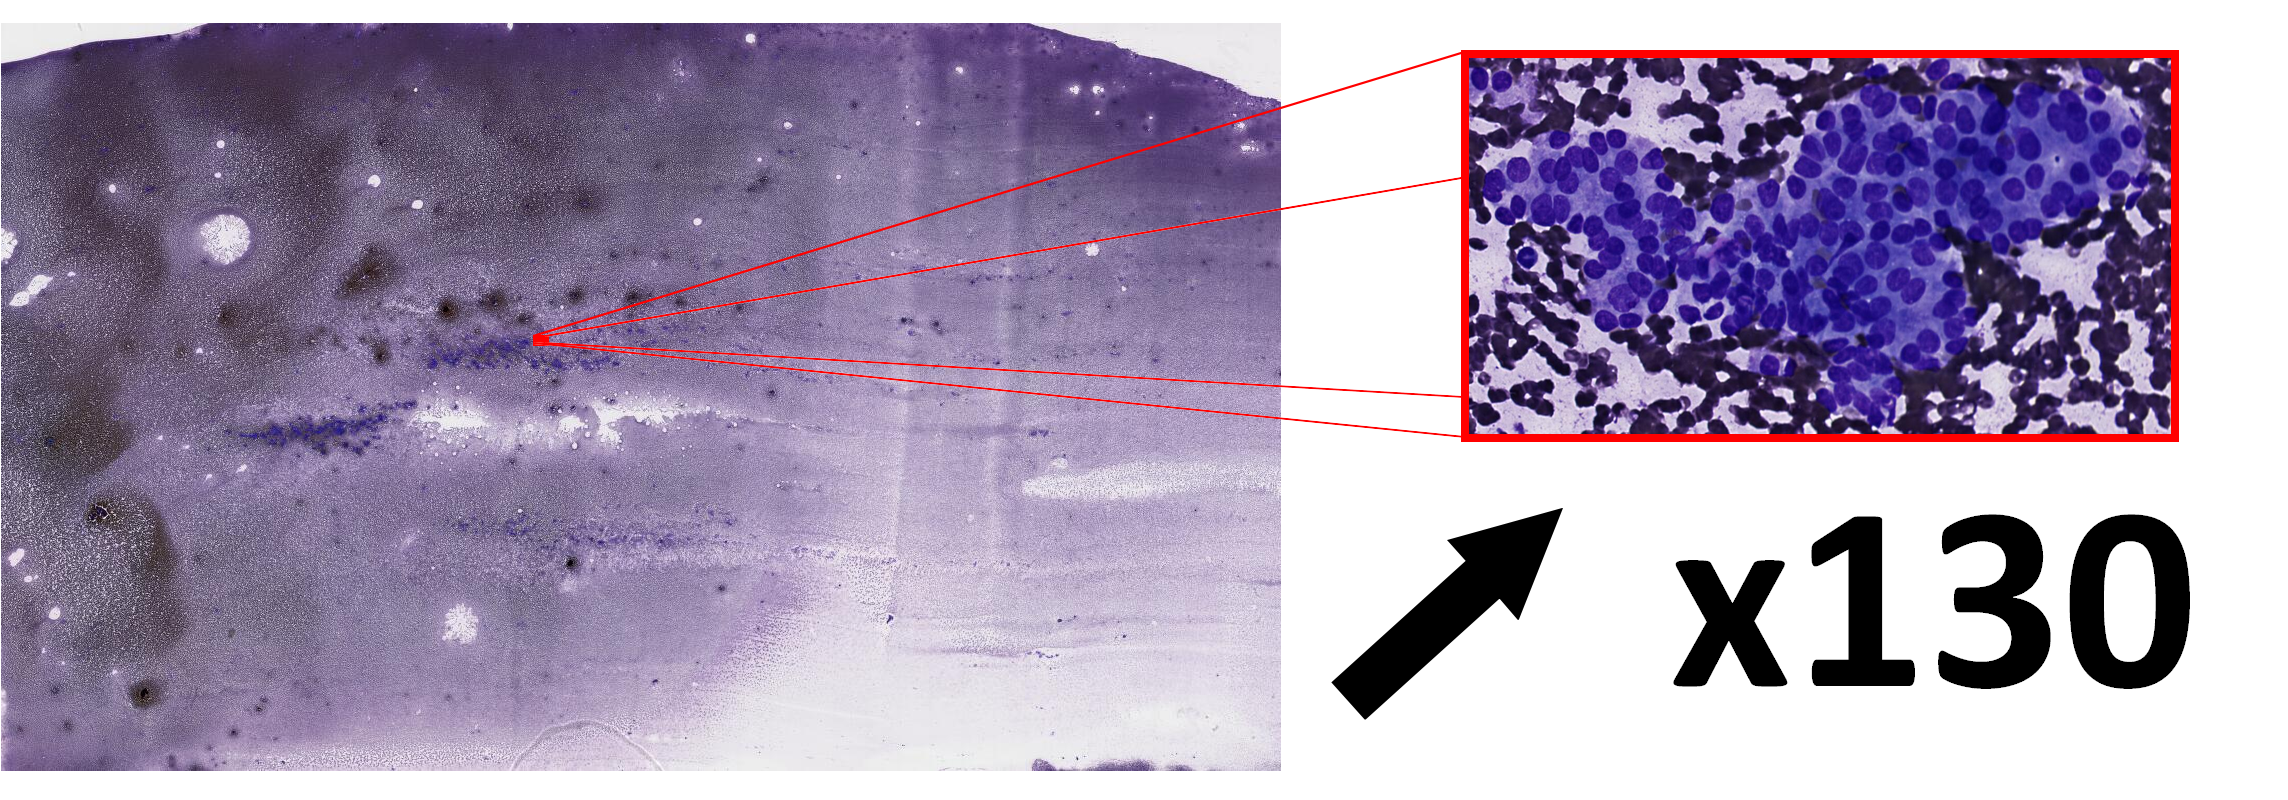
\includegraphics[scale=0.19]{images/whole-slide-dim.png}
	\caption{Microscope slide smeared with thyroid cell samples (15 gigapixels).}
	\end{figure}
	\vfill
\end{frame}

\begin{frame}{Context}
	\vfill
	\begin{figure}[h]
	\center
	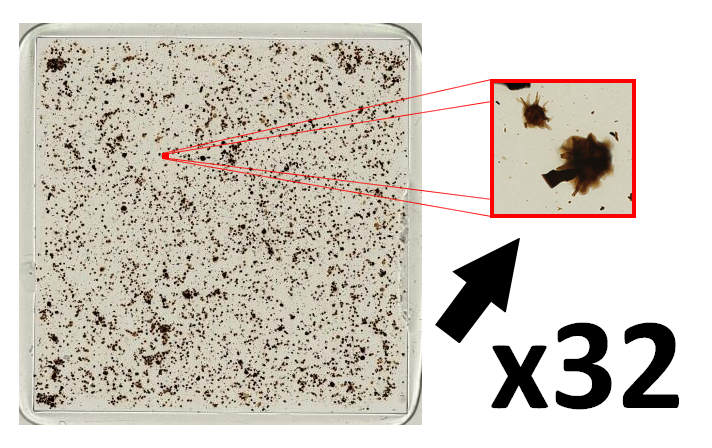
\includegraphics[scale=0.95]{images/whole-slide-geo-2.png}
	\caption{Microscope slide smeared with core samples (11 gigapixels).}
	\end{figure}
	\vfill
\end{frame}

\begin{frame}{Context}
	\vfill
	\begin{figure}[h]
	\center
	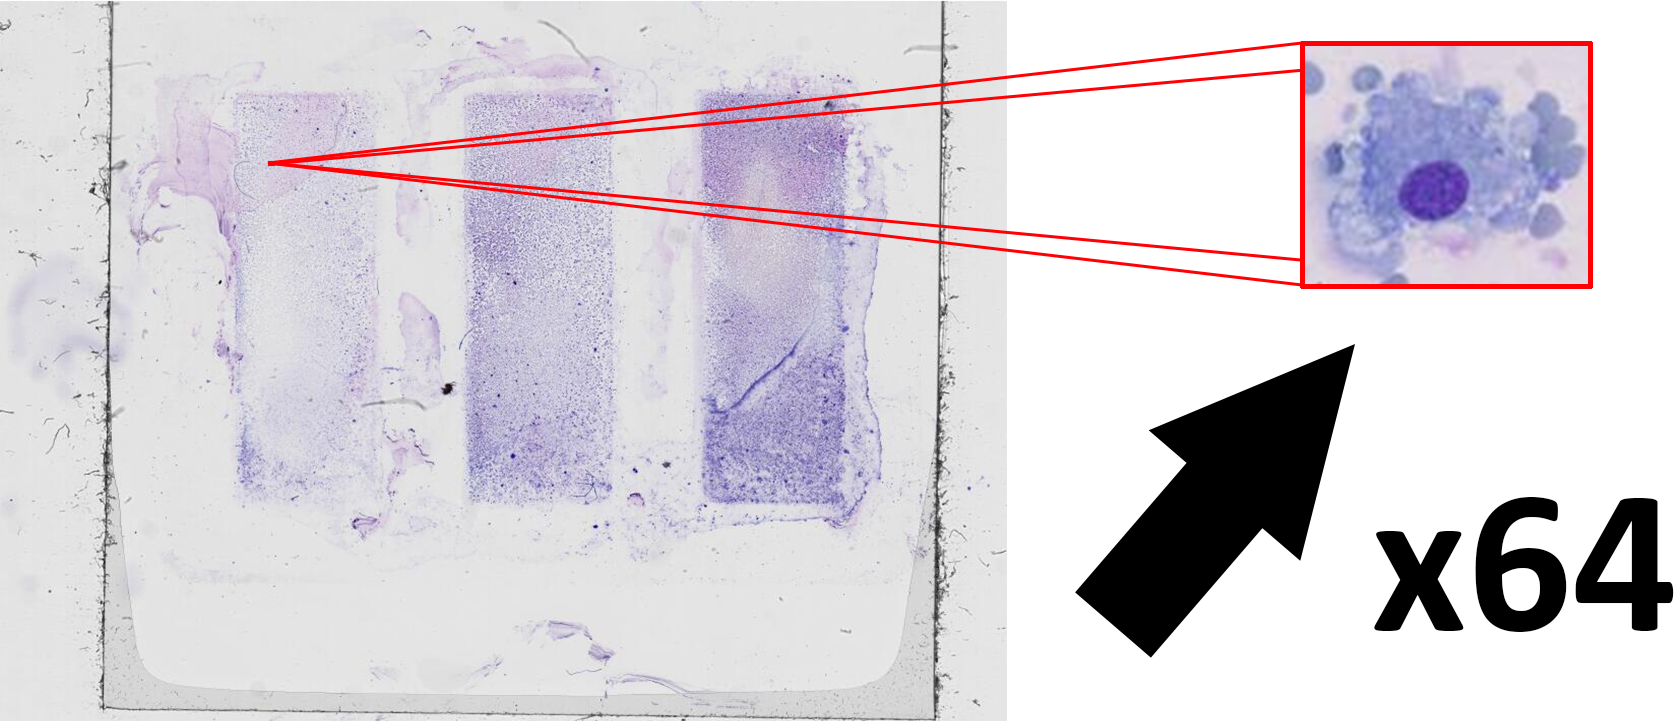
\includegraphics[scale=0.78]{images/whole-slide-lung-2.png}
	\caption{Microscope slide smeared with lung cell samples (3 gigapixels).}
	\end{figure}
	\vfill
\end{frame}

\begin{frame}{Context}
	\begin{itemize}
		\item Huge slides usually \textbf{analysed manually} !
		\item Machine learning (ML) and image processing (IP) could be used to assist humans
		\item Problems of \textbf{object detection and classification}
	\end{itemize}
\end{frame}


\begin{frame}{SLDC: framework}

	\textit{SLDC} is an \textbf{open-source Python framework} created for accelerating development of large image analysis workflows. 
	
	\vfill

	\textbf{How ?}
	\begin{itemize}

		\item It encapsulates problem-independent logic (parallelism, memory limitation due to large images handling,…)

		\item It provides a concise way of declaring problem dependant components (segmentation, object classification,…)

	\end{itemize}

\end{frame}

\begin{frame}{SLDC: features}
	\begin{itemize}
	
		\item \textbf{Tile-based processing} to avoid loading a full image into memory
		
		\item Several level of \textbf{parallelism}: tiles, objects, images,...
		
		\item A \textbf{customizable logging system} providing a rich feedback about the execution
		
		\item \textbf{Effortless integration} with other Python libraries: scikit-learn (ML), open-cv (IP), PyCuda (GPU),...
		
		\item \textbf{Builder components} providing an easy way of constructing complex workflows
		
	\end{itemize}
\end{frame}

\begin{frame}{SLDC: how it works}
	\begin{figure}
		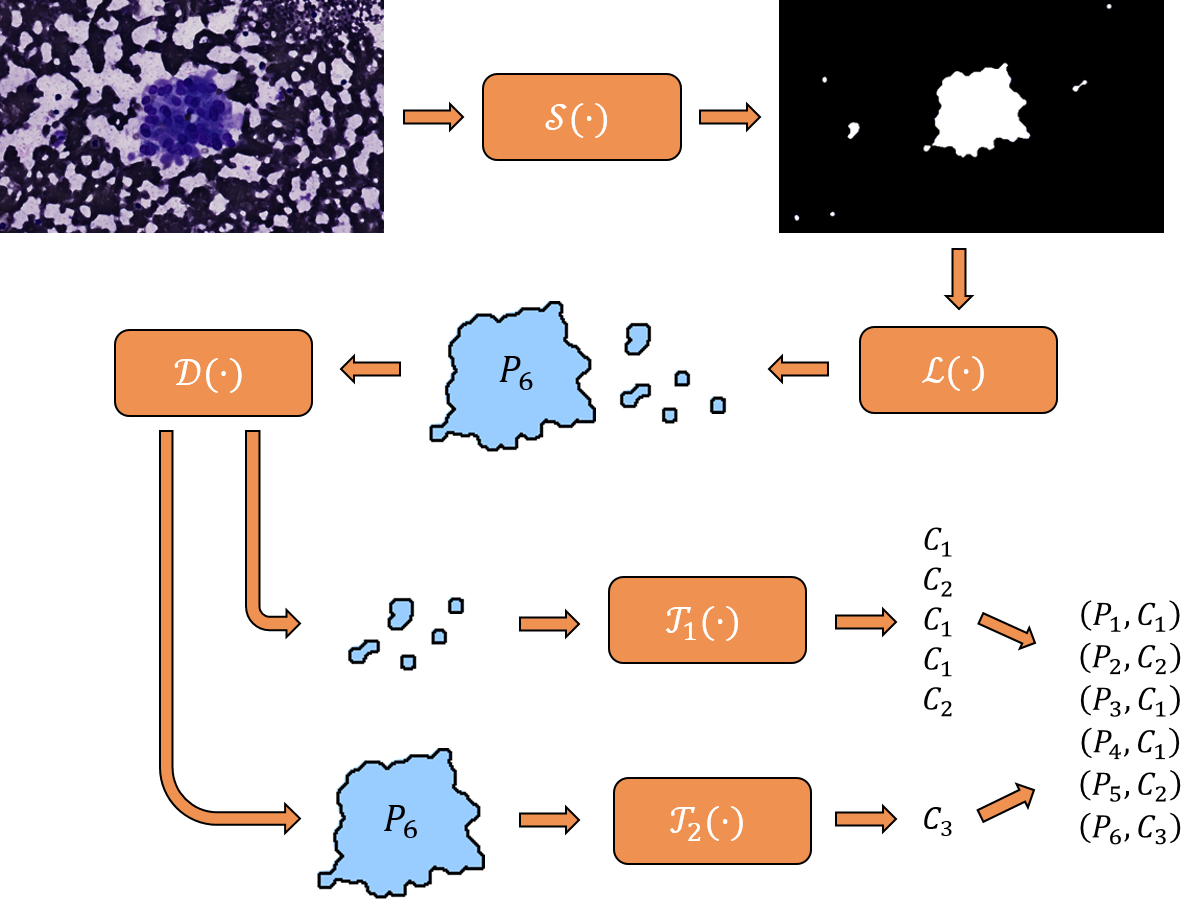
\includegraphics[scale=0.45]{images/workflow_illustration.png}
	\end{figure}
\end{frame}


\begin{frame}{SLDC at work: thyroid case}
	\begin{center}	
		Aim: detect \textbf{cells with inclusion} and \textbf{proliferative architectural patterns}
	\end{center}
	\begin{figure}
		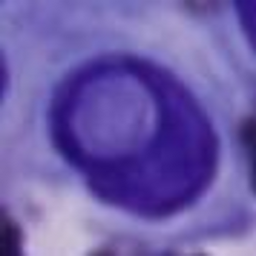
\includegraphics[scale=0.35]{images/incl1.png}
		\hspace{1cm}
		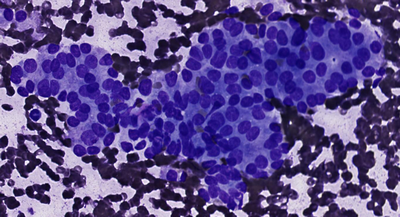
\includegraphics[scale=0.55]{images/prolif_pattern_1.png}
	\end{figure}
\end{frame}

\begin{frame}{SLDC at work: Cytomine}
	
\includegraphics[scale=0.09]{images/cytomine_typo.png} is a web-based environment enabling collaborative multi-gigapixel image analysis.  \footnotesize{(Website: \url{www.cytomine.be}. Marée \& al., Bioinformatics; 2016)}.\\
	\vspace*{0.01in}
	\hspace*{-1.5in}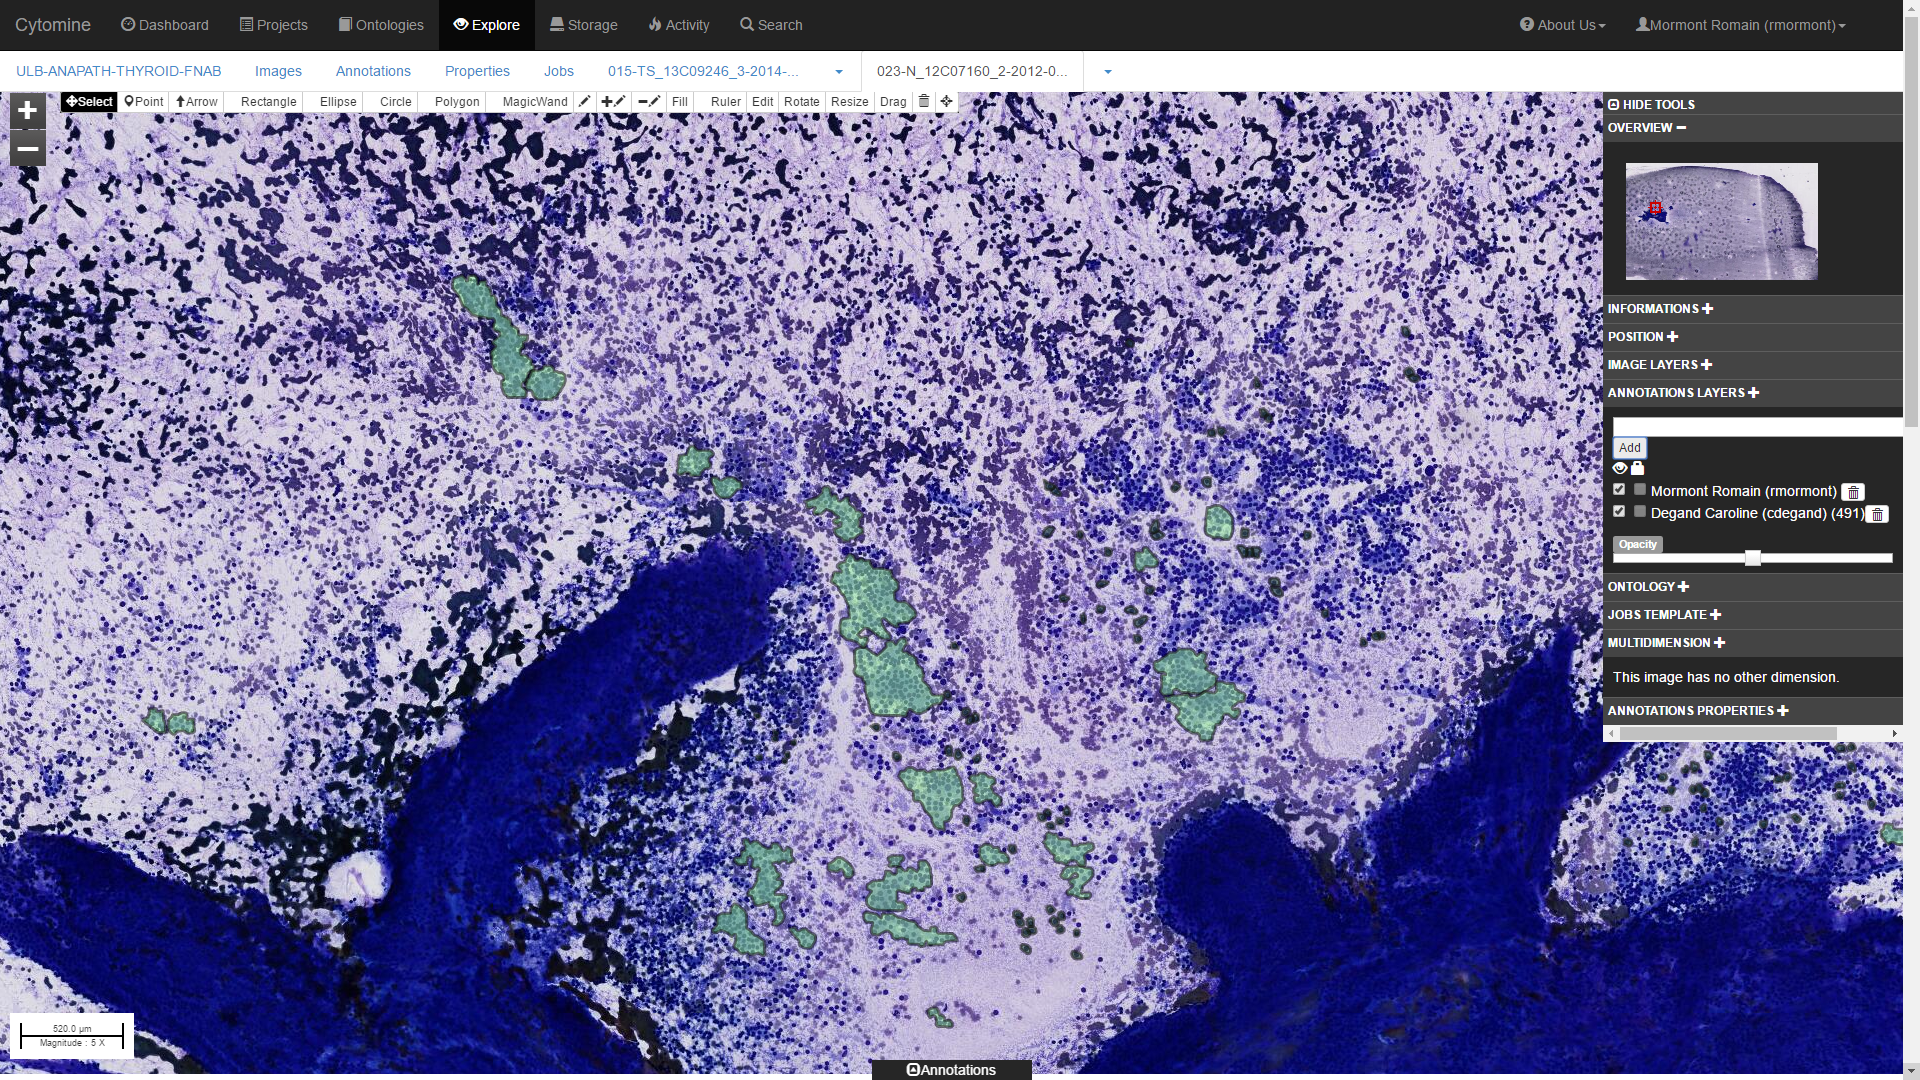
\includegraphics[scale=0.24]{images/cytomine.png}
\end{frame}

\begin{frame}{SLDC at work: data}
	\begin{itemize}
		\item \textbf{84 images} with size ranging from 4 to 18 gigapixels
		\item \textbf{68 annotated images} 
		\item \textbf{5921 labelled annotations} made by cytopathologists\footnote[frame]{Team of Pr. Isabelle Salmon, Department of Pathology, Faculty of Medecine, ULB}
	\end{itemize}

	\begin{figure}
		\center
		\subfigure[Annot. per group]{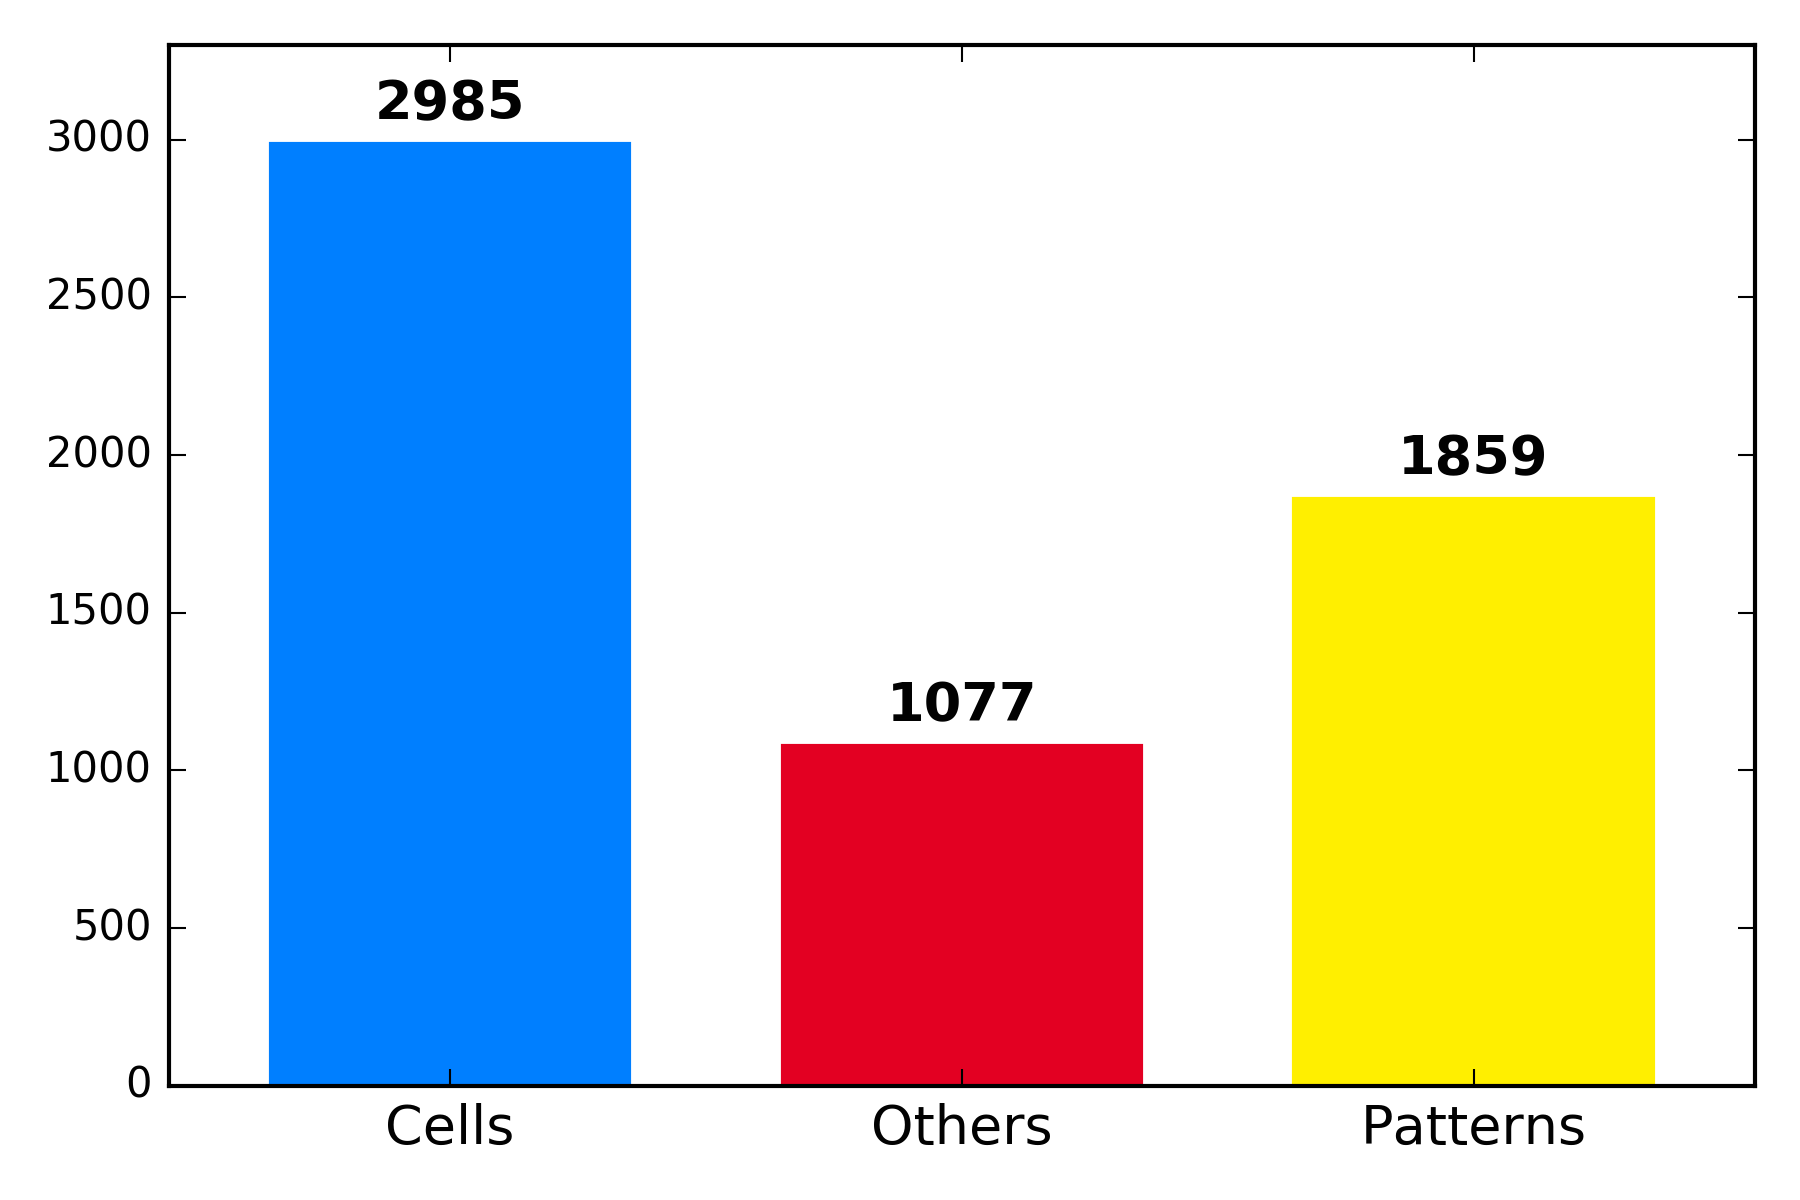
\includegraphics[scale=0.35]{images/counts_all_grouped.png}}
		\subfigure[Annot. per term]{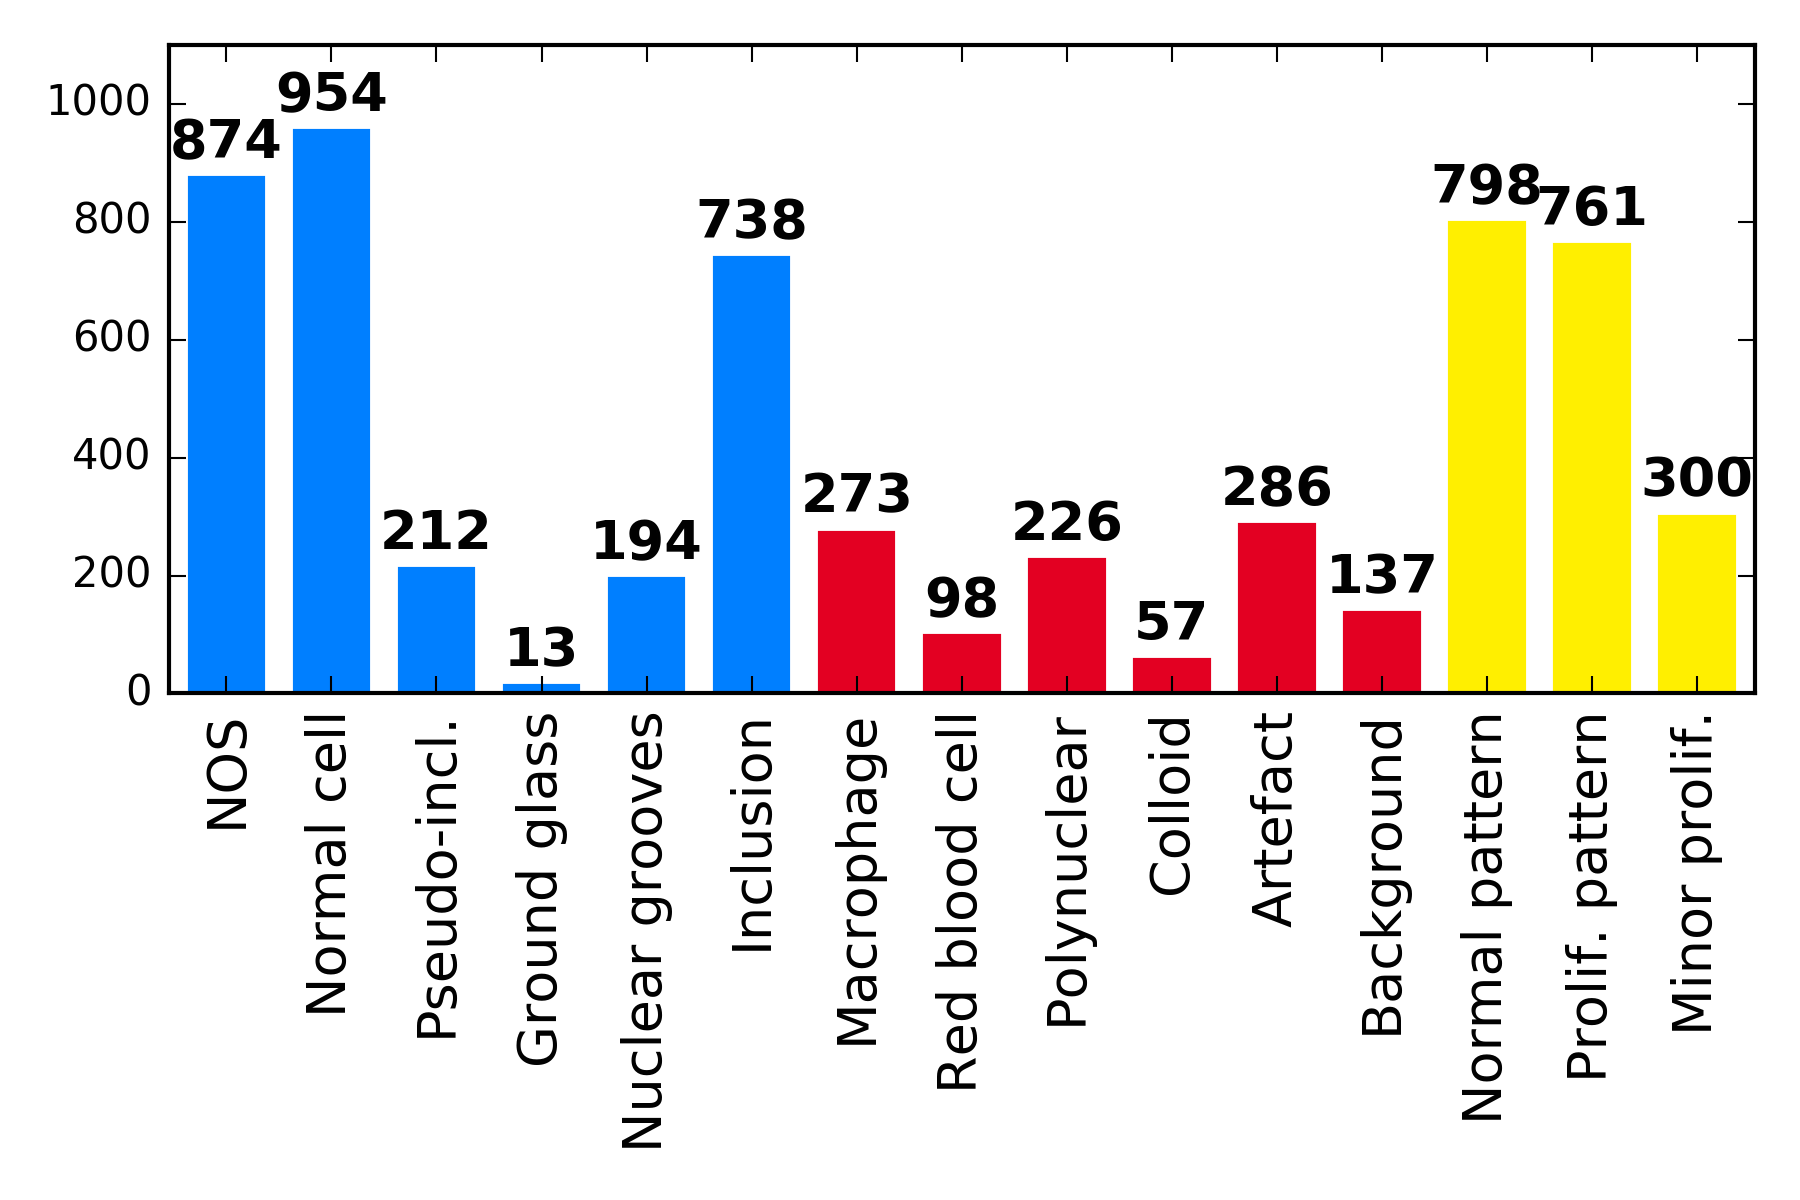
\includegraphics[scale=0.35]{images/counts_all.png}}
	\end{figure}
\end{frame}

\begin{frame}{SLDC at work: data (cont'd)}
	\begin{figure}
		\center
		\subfigure[Pattern annot. per group]{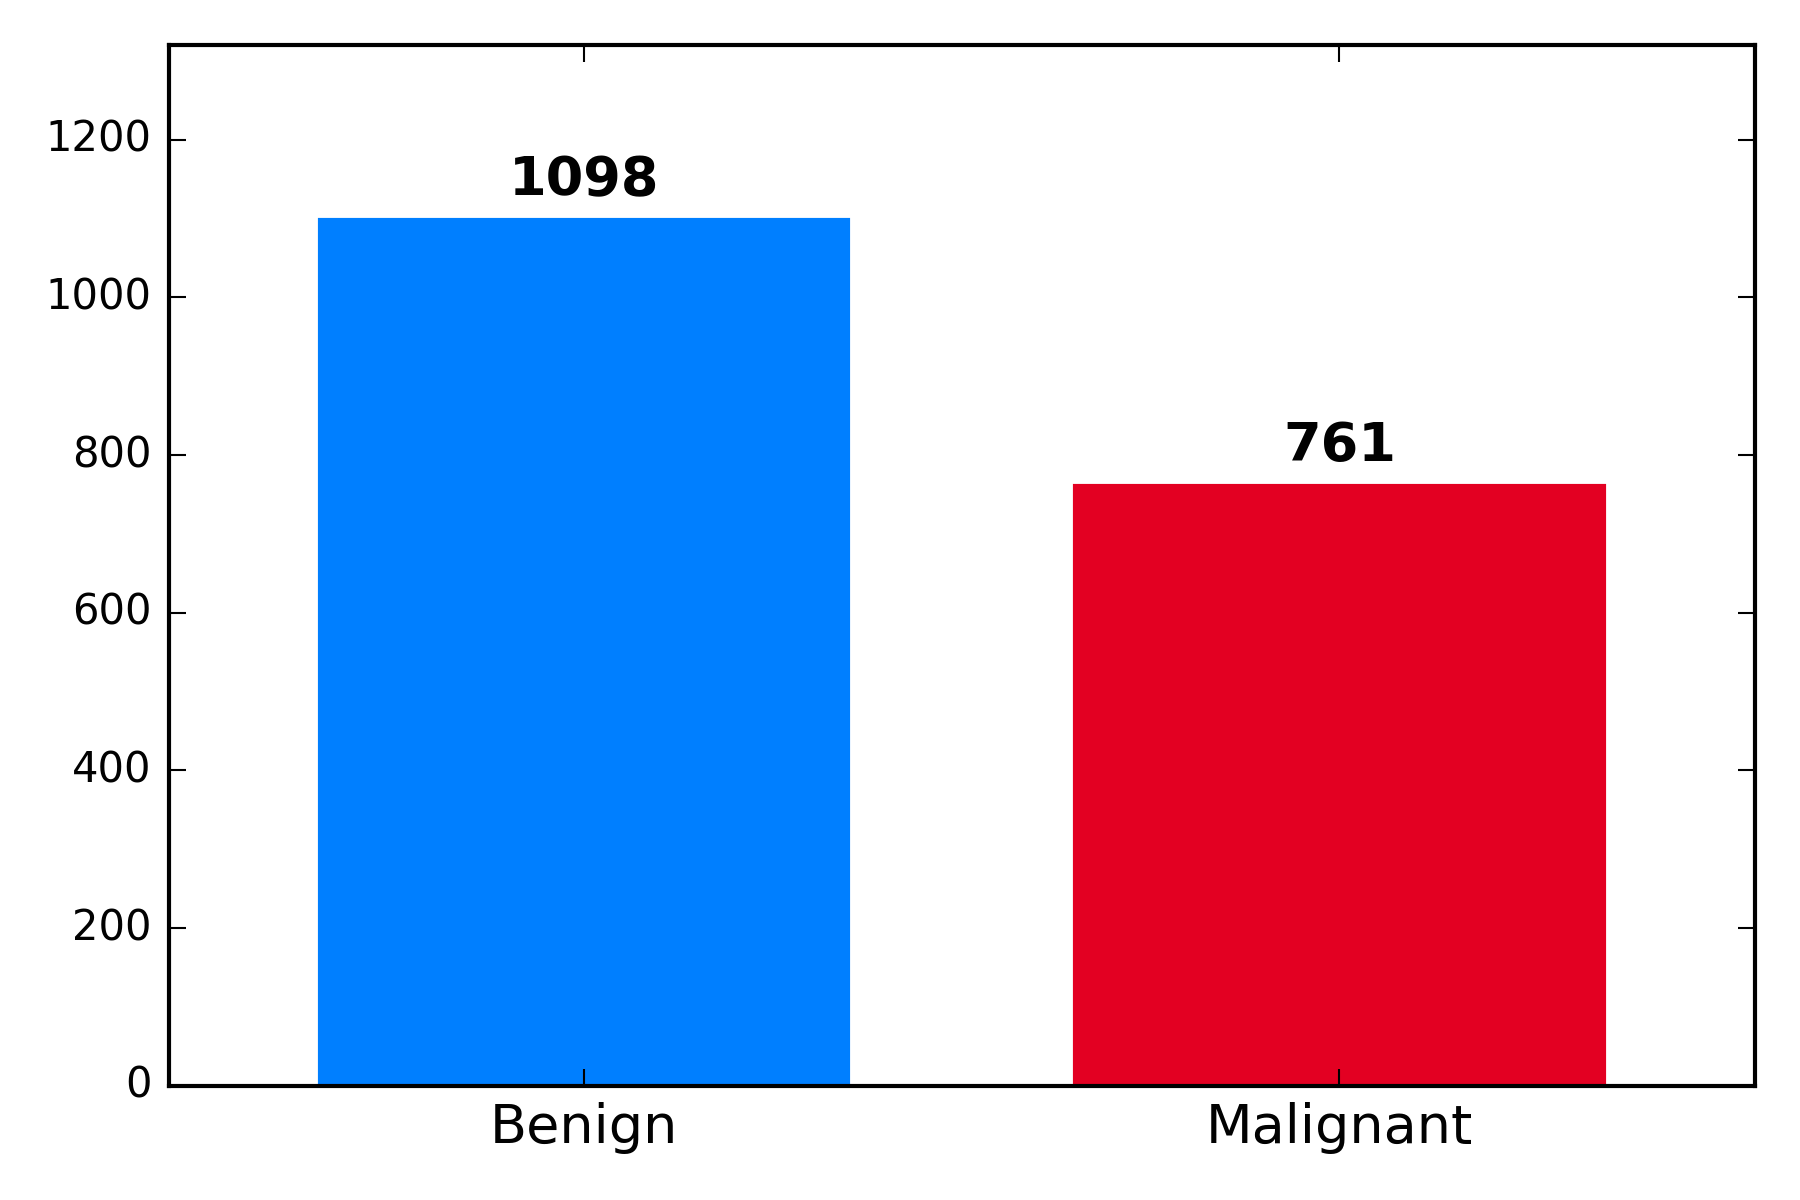
\includegraphics[scale=0.32]{images/counts_patterns_grouped.png}}
		\subfigure[Pattern annot. per term]{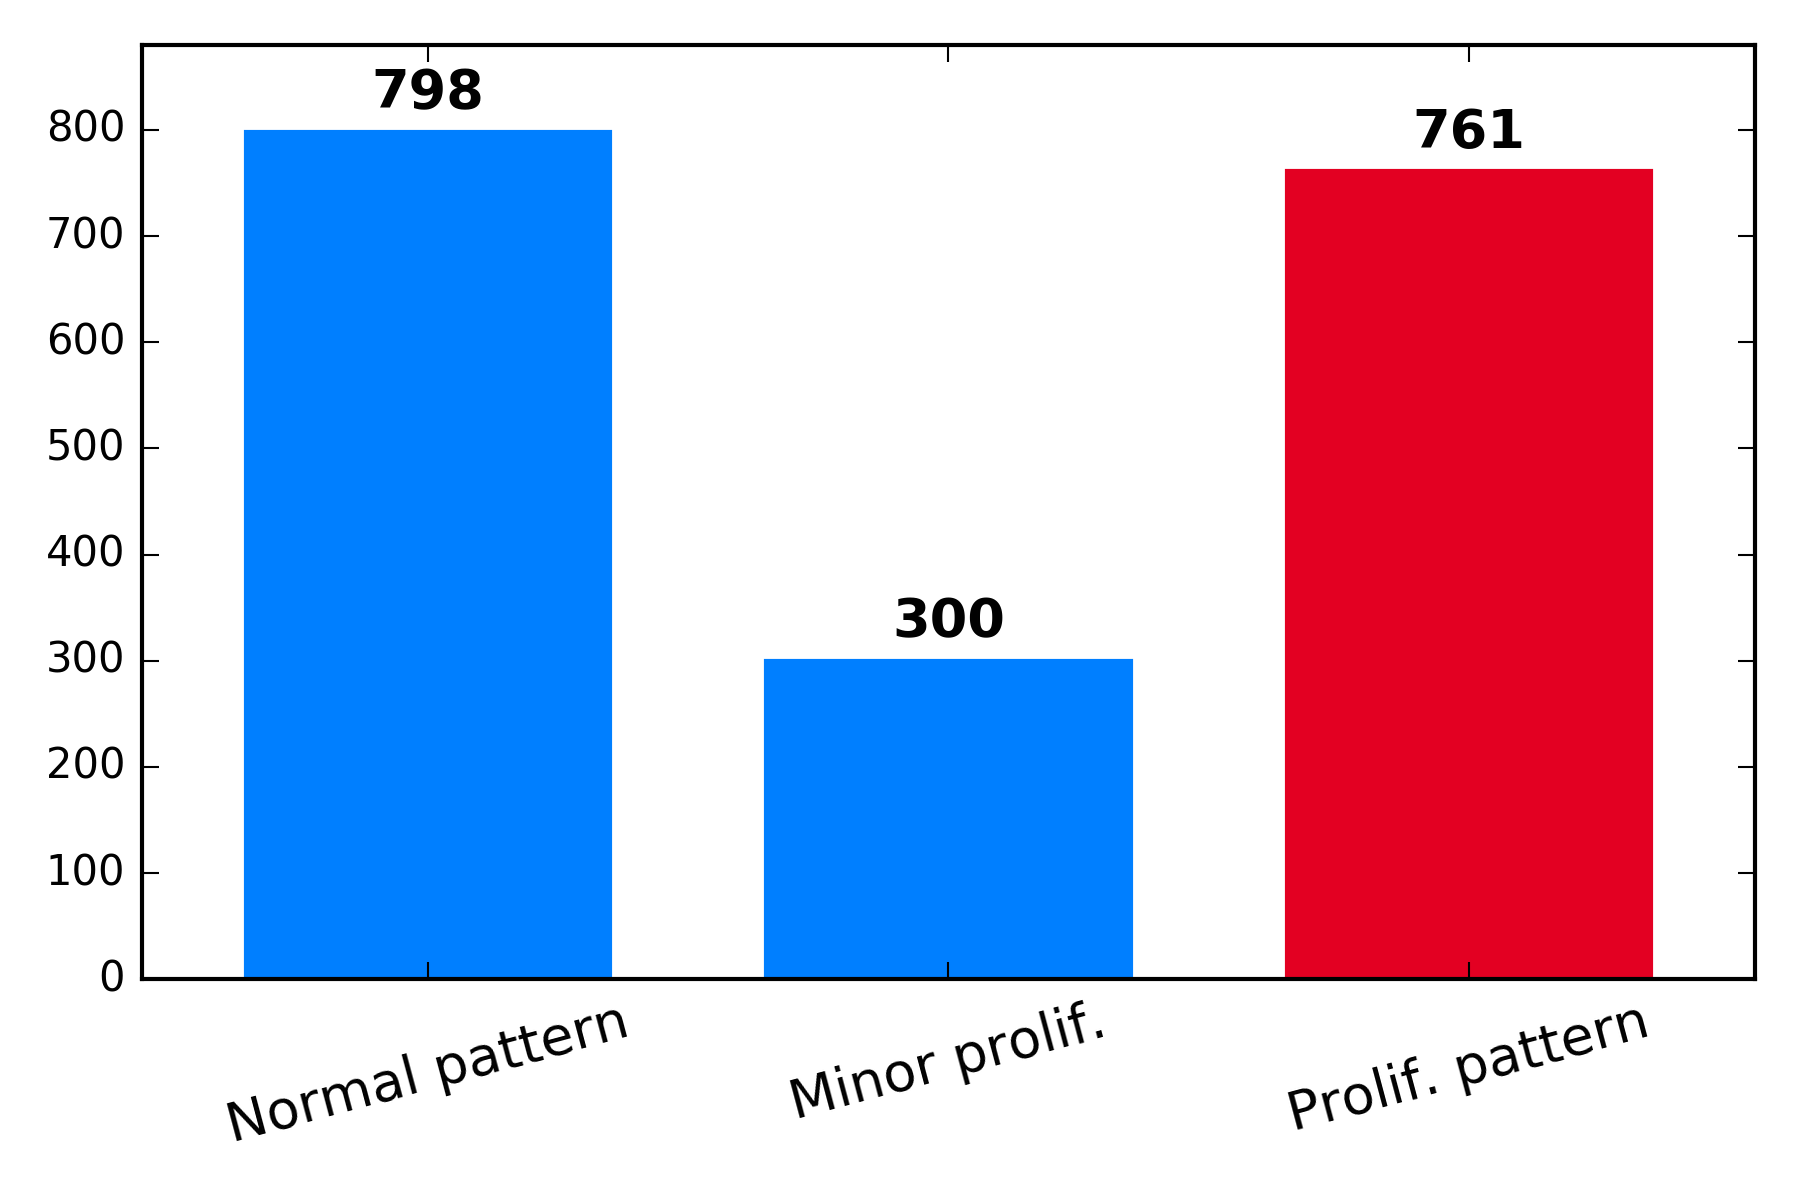
\includegraphics[scale=0.32]{images/counts_patterns.png}}\\
		\subfigure[Proliferative (malignant)]{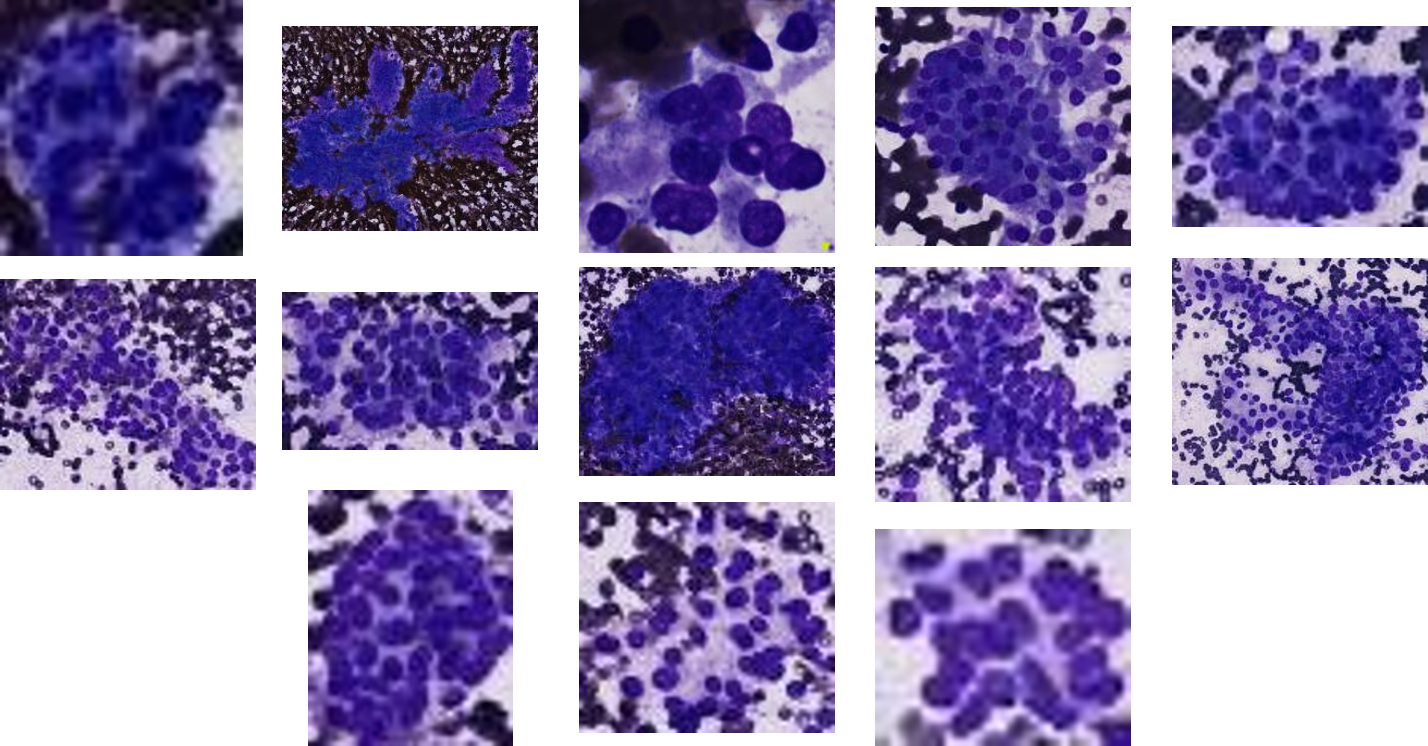
\includegraphics[scale=0.1]{images/all_prolif.png}}
		\hspace*{.5cm}
		\subfigure[Normal patterns (benign)]{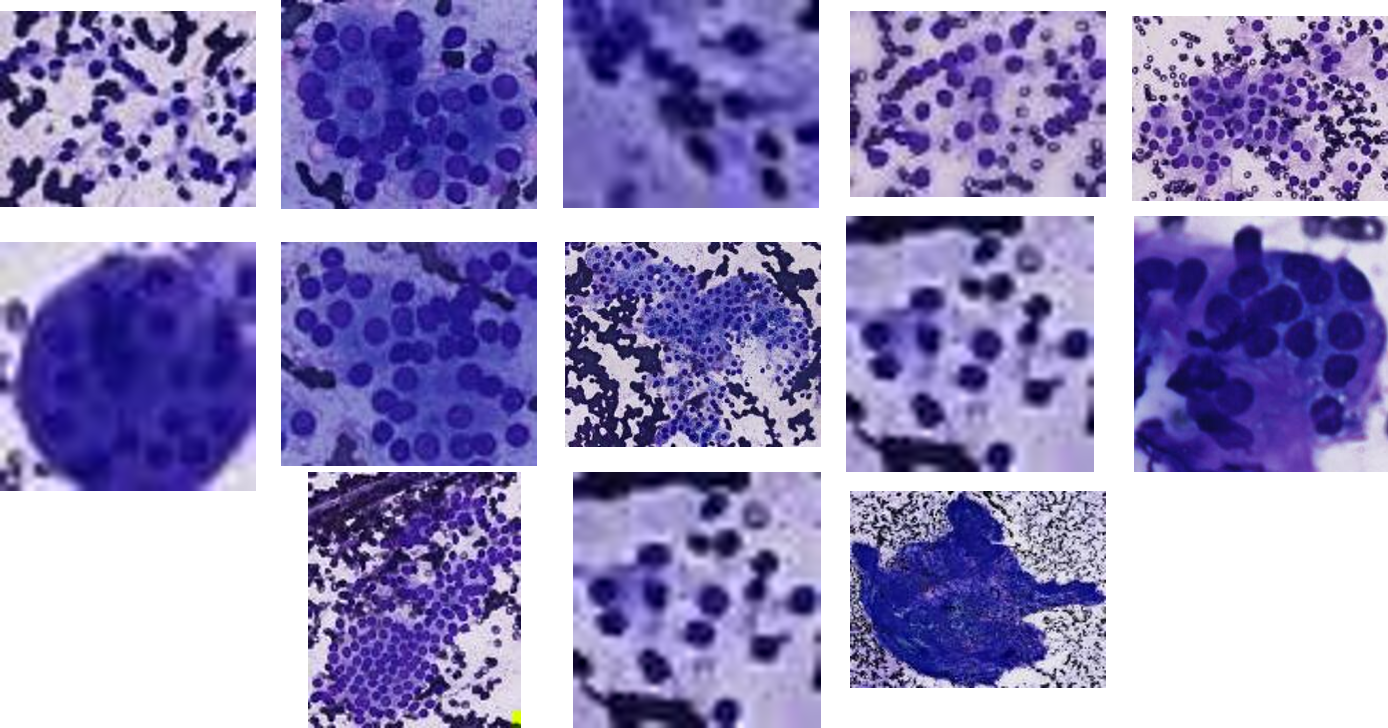
\includegraphics[scale=0.1]{images/all_norm_patterns.png}}
	\end{figure}
\end{frame}

\begin{frame}{SLDC at work: data (cont'd)}
	\begin{figure}
		\subfigure[Cell annot. per group]{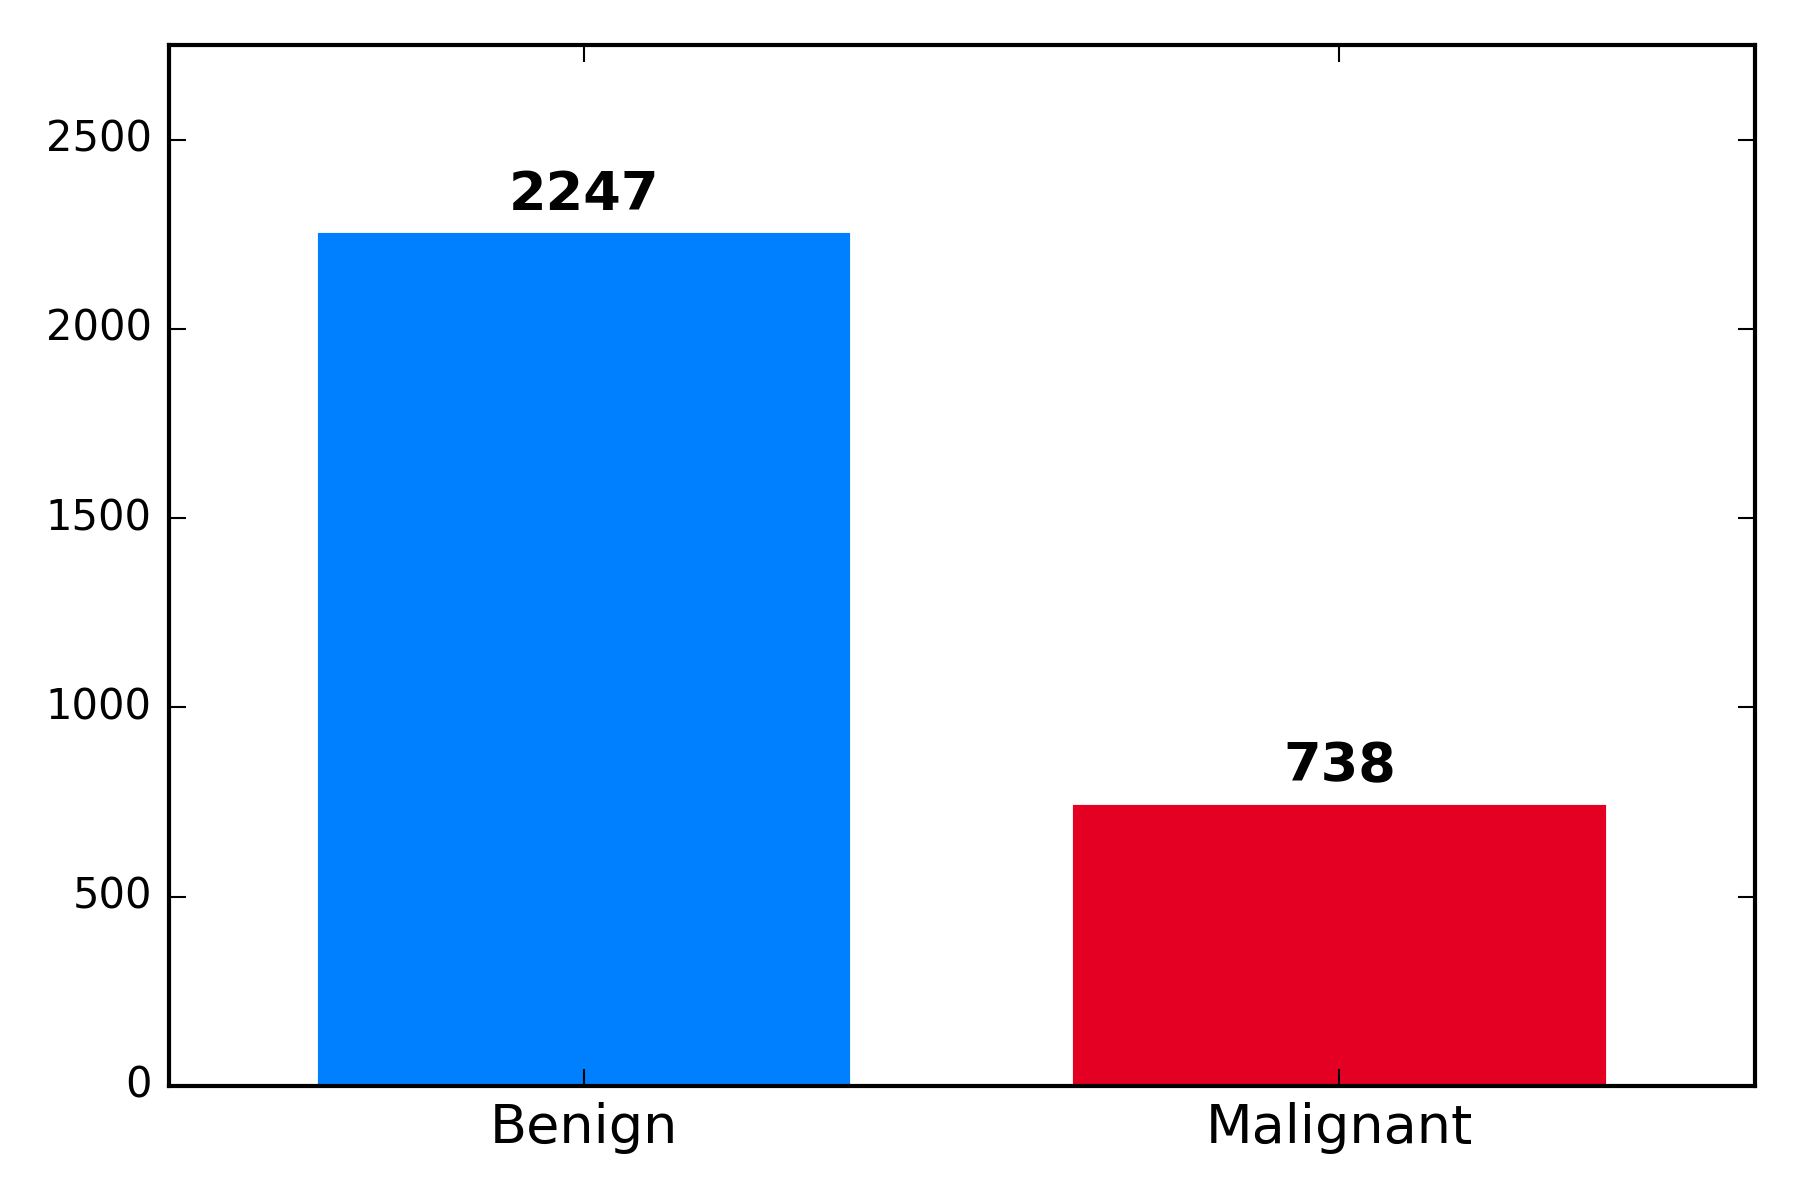
\includegraphics[scale=0.32]{images/counts_cells_grouped.png}}
		\subfigure[Cell annot. per term]{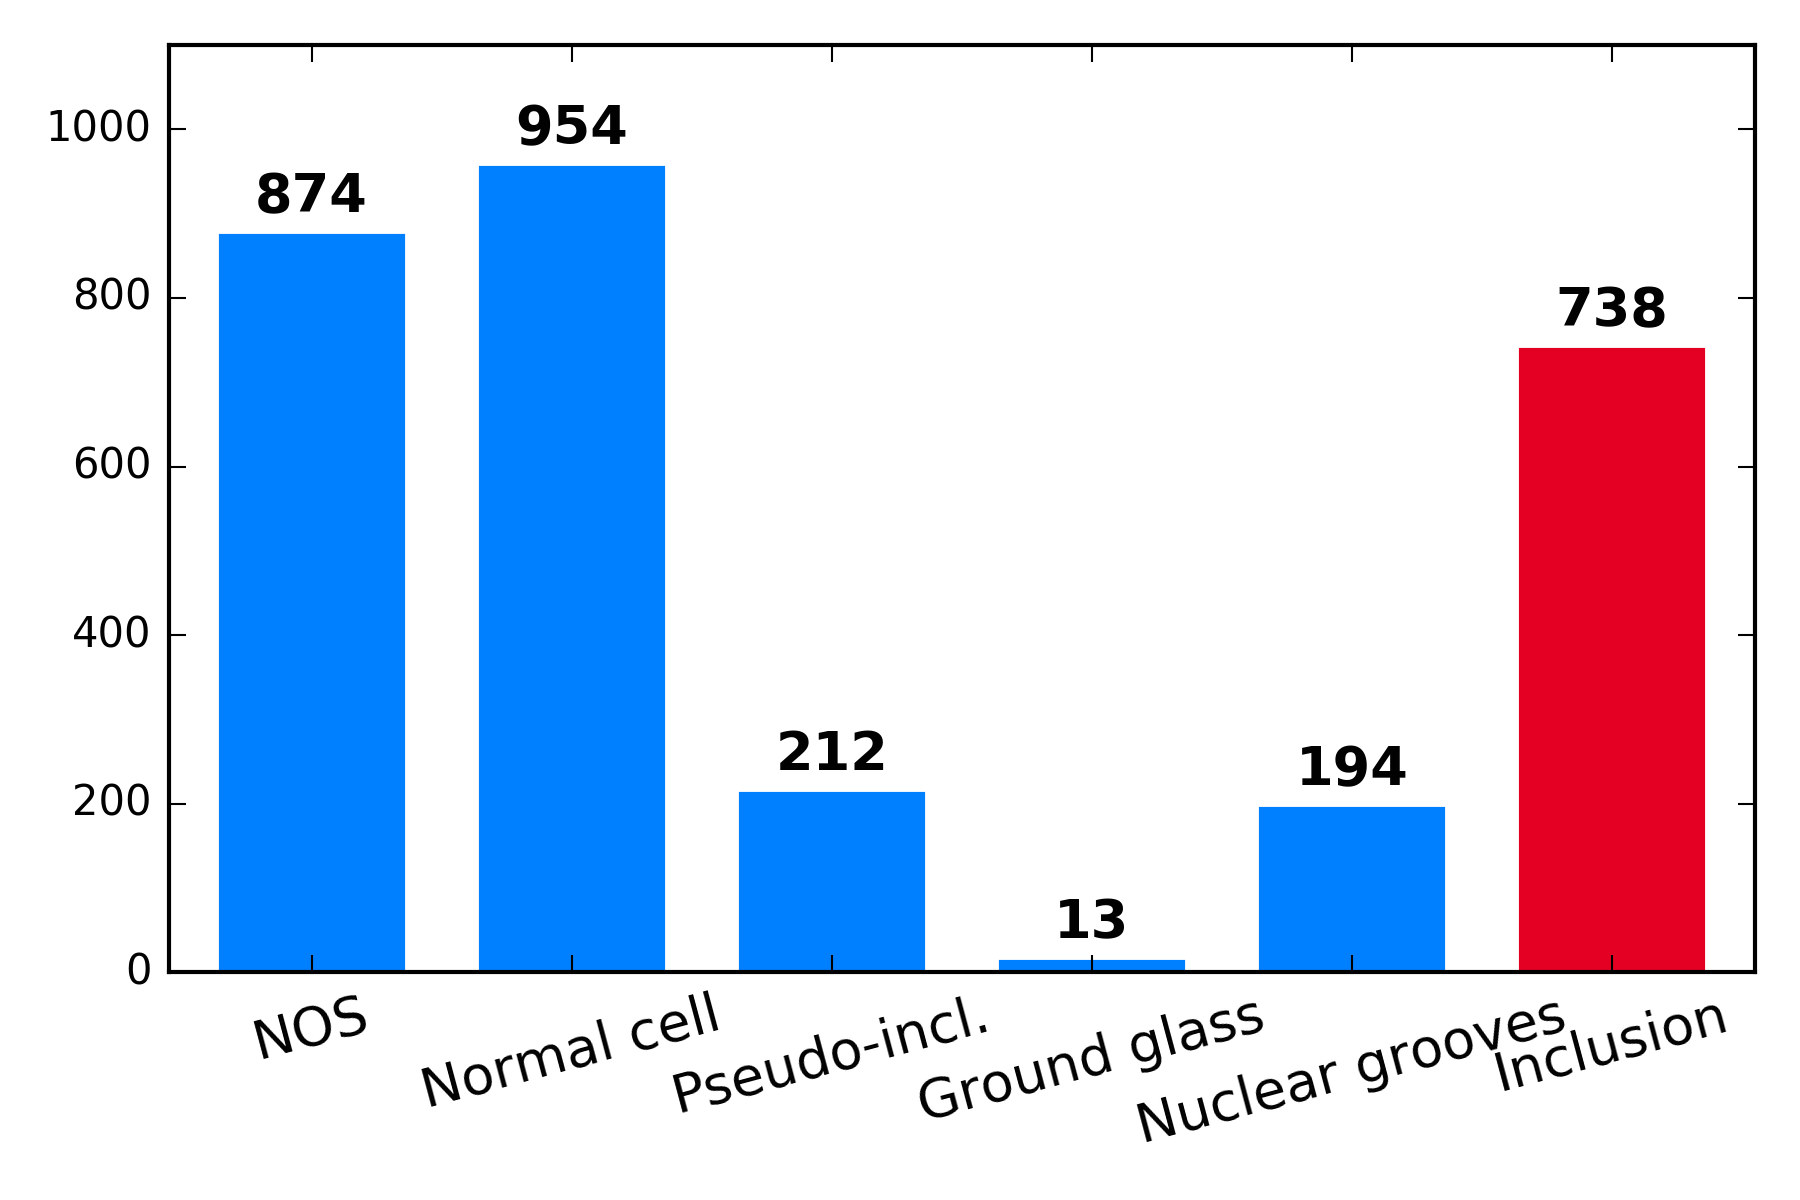
\includegraphics[scale=0.32]{images/counts_cells.png}}\\
		\subfigure[Cells with incl. (malignant)]{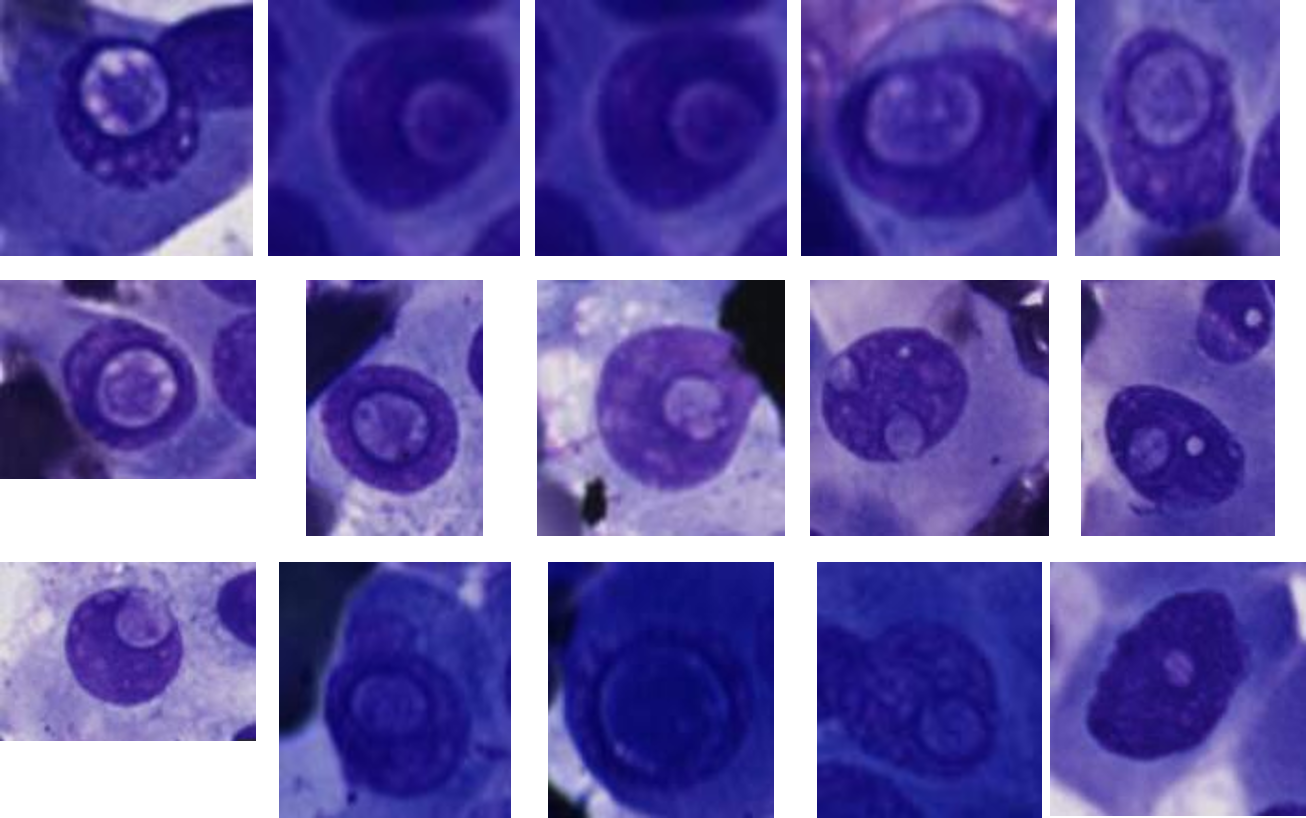
\includegraphics[scale=0.1]{images/all_incl.png}}
		\hspace*{.5cm}
		\subfigure[Normal cells (benign)]{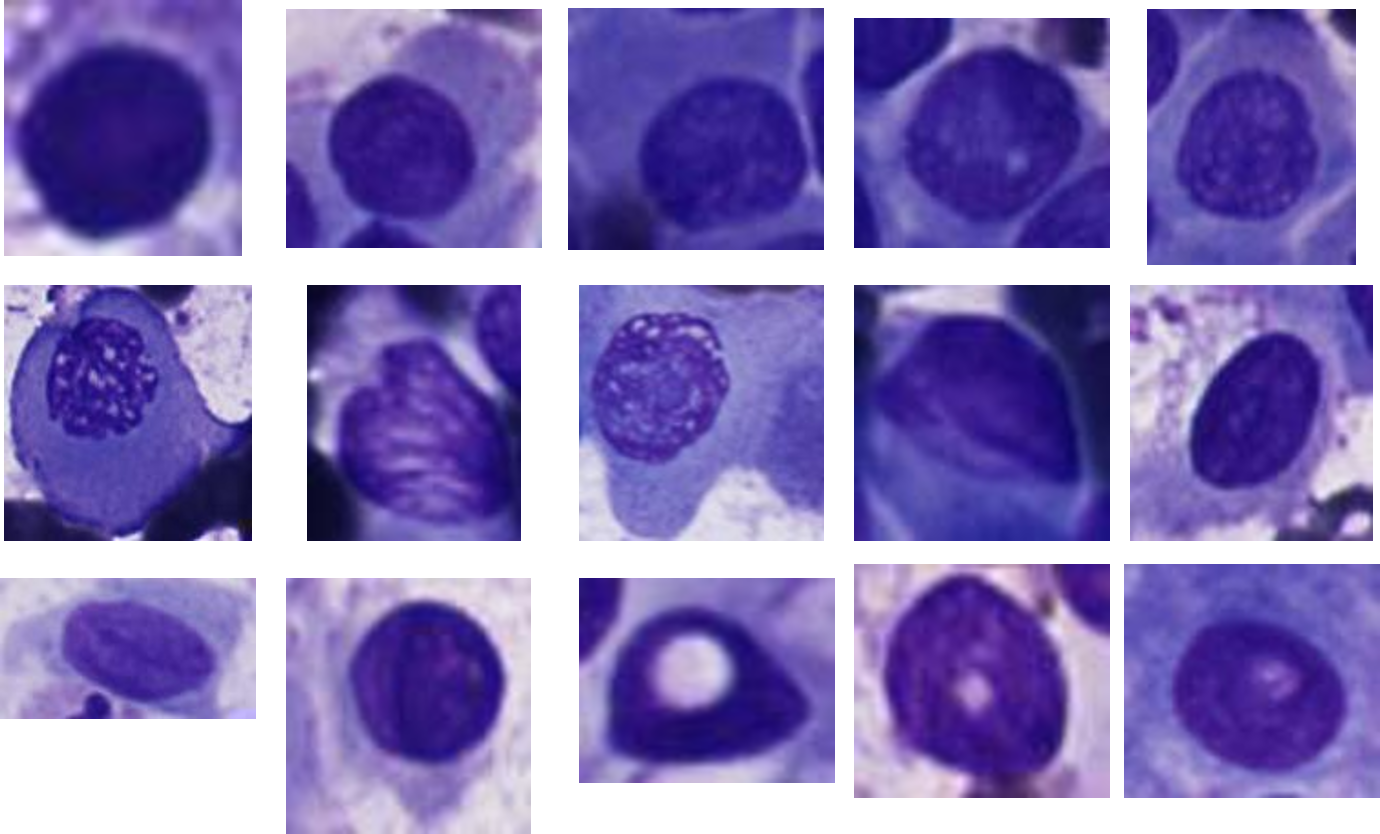
\includegraphics[scale=0.1]{images/all_norm_cells.png}}
	\end{figure}
\end{frame}

\begin{frame}{SLDC at work: workflow}
	\begin{figure}
		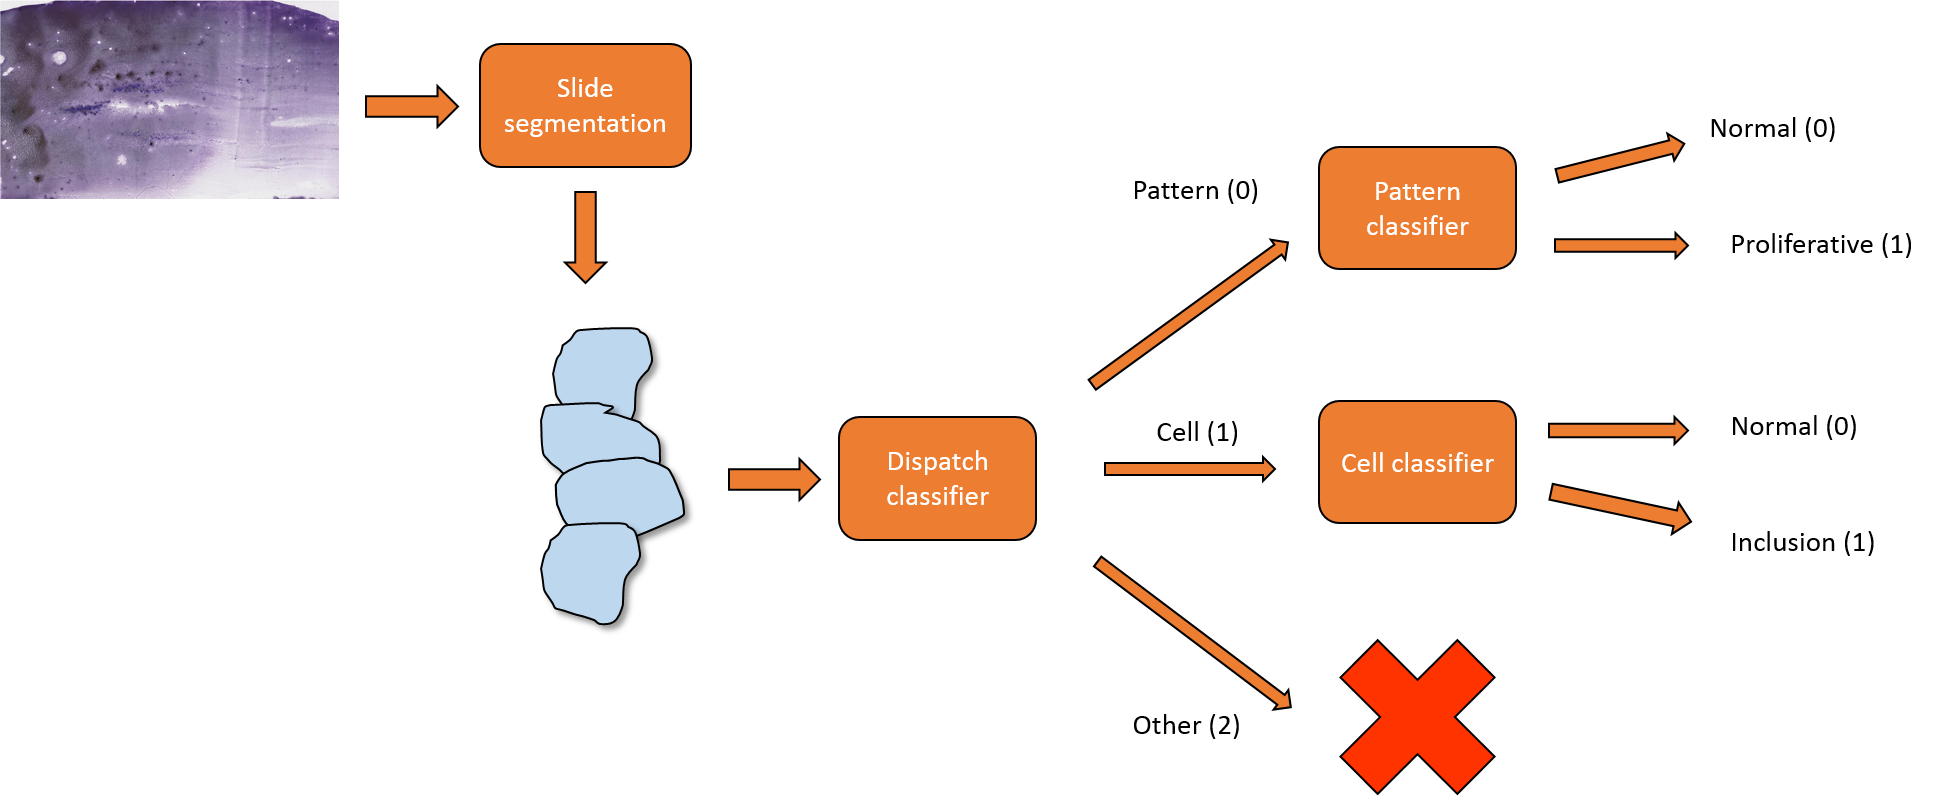
\includegraphics[scale=0.35]{images/thyroid_workflow_1.png}
	\end{figure}
\end{frame}

\begin{frame}{SLDC at work: workflow (cont'd)}
	\begin{figure}
		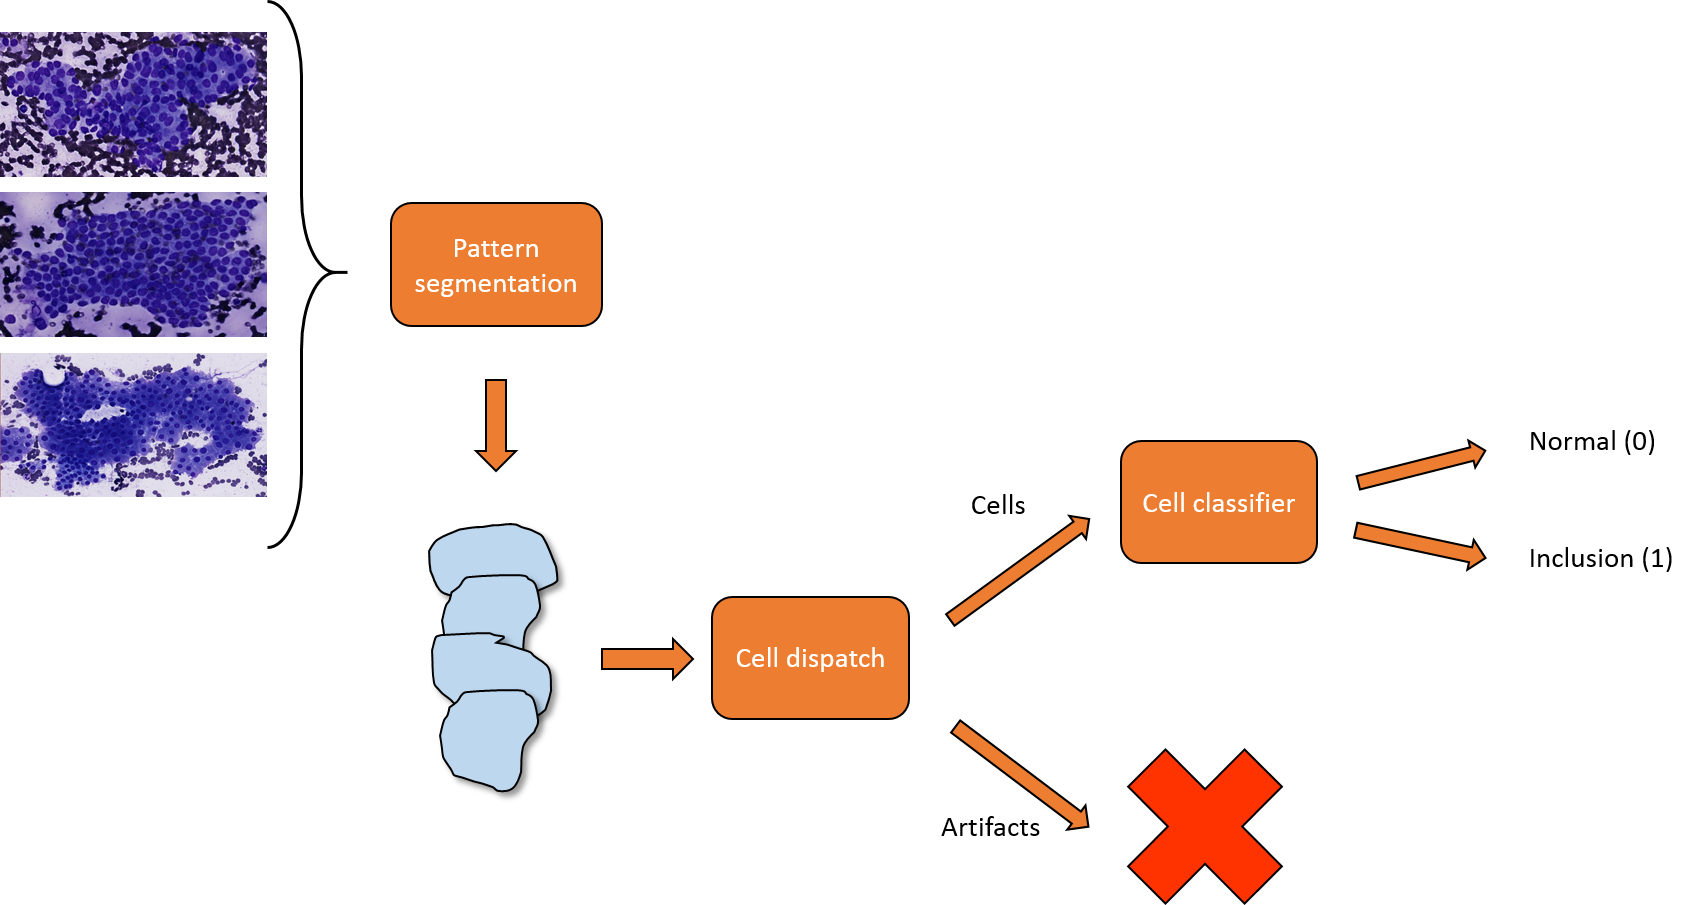
\includegraphics[scale=0.4]{images/thyroid_workflow_2.png}
	\end{figure}
\end{frame}

\begin{frame}{SLDC at work: workflow (cont'd)}

	Classification is performed based on the detected object's crop image using \textbf{random subwindows and extremely randomized trees}\footnote[frame]{Marée et al., Pattern Recognition Letters ; 2016}.
	
	\vfill
	
	\begin{columns}
		\footnotesize
		\begin{column}{0.492\linewidth}
			
			\textbf{Cell with inclusion vs. normal cells}: 
			
			\vspace{0.4cm}
			
			\begin{tabular}{rc}
			  Accuracy:  & 0.8523 \\
			  Precision: & 0.6310 \\
			  Recall:    & \textcolor{red}{0.4930} \\
			\end{tabular}
			
			\vspace{0.4cm}
			
			\begin{tabular}{c|ccc}
				& Normal & Inclusion \\
				\hline
				Normal & 881 & 62 \\
				Inclusion & 109 & 106 \\
			\end{tabular}

		\end{column}
		
		\begin{column}{0.49\linewidth}
		
			\textbf{Proliferative vs. normal patterns}:
			 
			\vspace{0.4cm}

			\begin{tabular}{rc}
			  Accuracy:  & 0.8625 \\
			  Precision: & 0.8363 \\
			  Recall:    & 0.9493 \\
			\end{tabular}
			
			\vspace{0.4cm}
			
			\begin{tabular}{c|ccc}
				& Normal & Prolif. \\
				\hline
				Normal & 158 & 55 \\
				Prolif. & 15 & 281 \\
			\end{tabular}
			
		\end{column}

	\end{columns}
	
\end{frame}

\begin{frame}{SLDC at work: results}
	\footnotesize
	\vspace*{-0.2cm}
	\begin{columns}
		\begin{column}{0.40\linewidth}
			\begin{figure}
				\center
				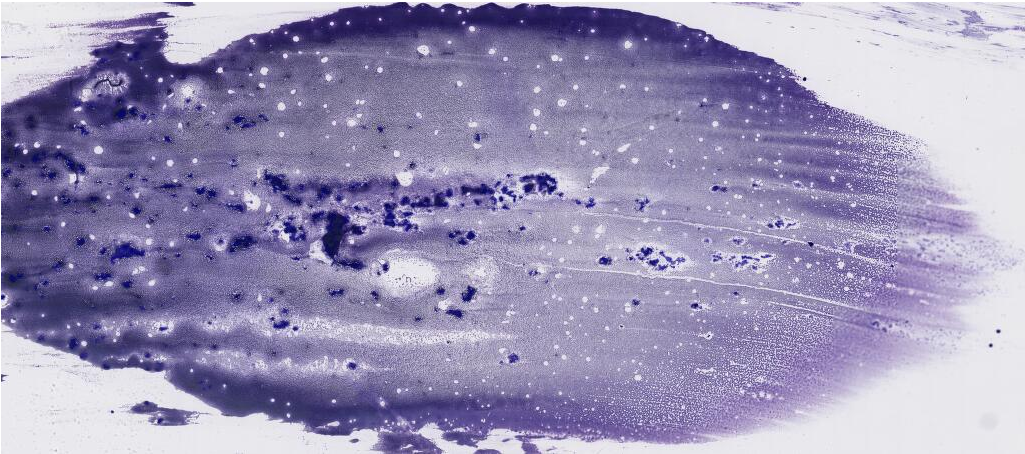
\includegraphics[scale=0.2]{images/728725.png}
				\caption{Size: 131072 $\times$ 57856}
			\end{figure}
		\end{column}
		\begin{column}{0.47\linewidth}
			\begin{tabular}{rl}
				Objects found: & \textbf{20046} \\
				Cells found: & 18966 \\
				Patterns found: & 1080 \\
				& \\
				Time (1st pass): & \textbf{7 min 30 sec} \\
				Time (2nd pass): & 1 h 10 min  \\
				Peak memory: & 138 Go \\
			\end{tabular}
		\end{column}
	\end{columns}
	\begin{columns}
		\begin{column}{0.40\linewidth}
			\begin{figure}
				\center
				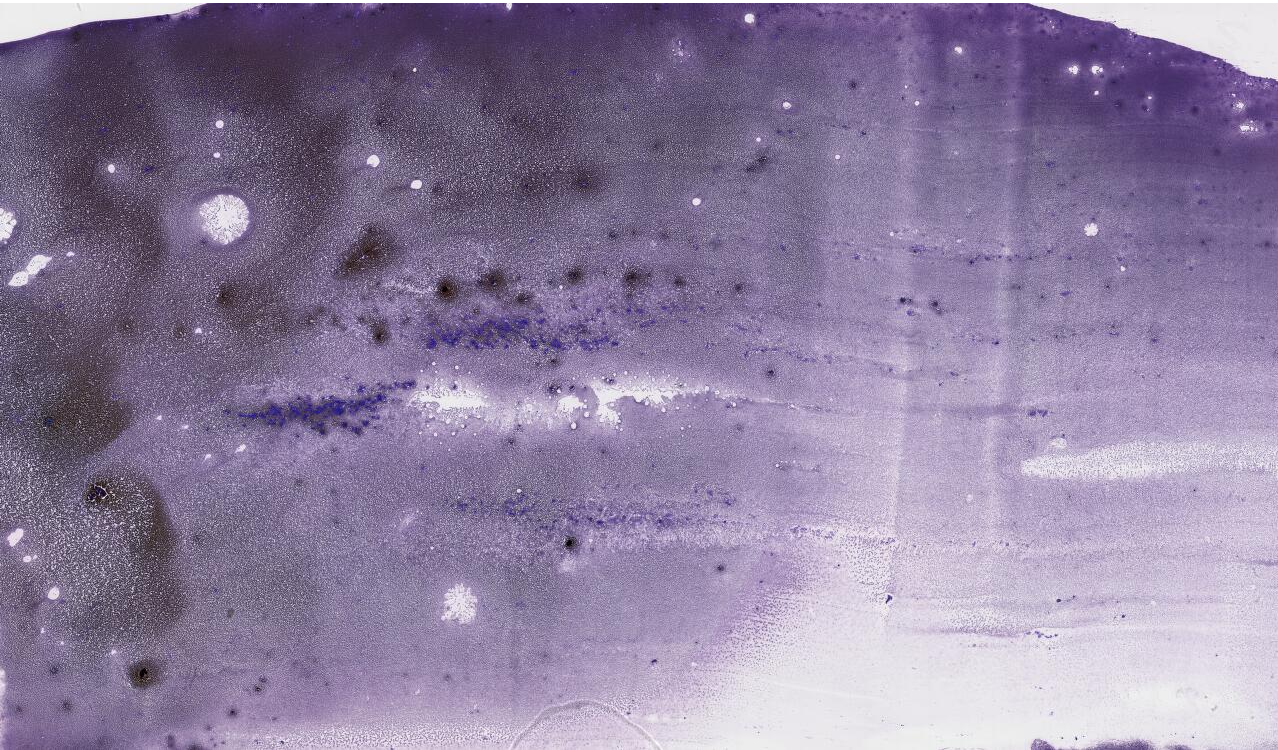
\includegraphics[scale=0.16]{images/716528.png}
				\caption{Size: 163840 $\times$ 95744}
			\end{figure}
		\end{column}
		\begin{column}{0.47\linewidth}
		\begin{tabular}{rl}
				Objects found: & \textbf{79063} \\
				Cells found: & 72740 \\
				Patterns found: & 6323 \\
				& \\
				Time (1st pass): & \textbf{18 min 20 sec} \\
				Time (2nd pass): & 4 h 50 min  \\
				Peak memory: & 178 Go \\
			\end{tabular}
		\end{column}
	\end{columns}
	
\end{frame}


\begin{frame}{Conclusion and future works}

	\begin{enumerate}
		\item Framework

		\begin{itemize}
			\item Production-ready !
			\item Open-source and generic.
			\item Still some minor improvements to make (parallelization, dispatching,...)
			\item \textbf{Feel free to use it}: {\small\url{https://github.com/waliens/sldc}}
		\end{itemize}
		
		\item Thyroid workflow:
		
		\begin{itemize}
			\item At this point, too many false positives.
			\item Need to improve the classifiers and the segmentation procedures
		\end{itemize}			
	\end{enumerate}

\end{frame}


\begin{frame}
	\vfill
	\begin{center}
		Thank you for your attention ! \\
		Any question ?
	\end{center}
	\vfill
\end{frame}

%% Bonus slides

\begin{frame}{SLDC: toy example}
	The aim is to detect circles in the following image. As a bonus, we want to know their center color.
	\vfill
	\begin{figure}
		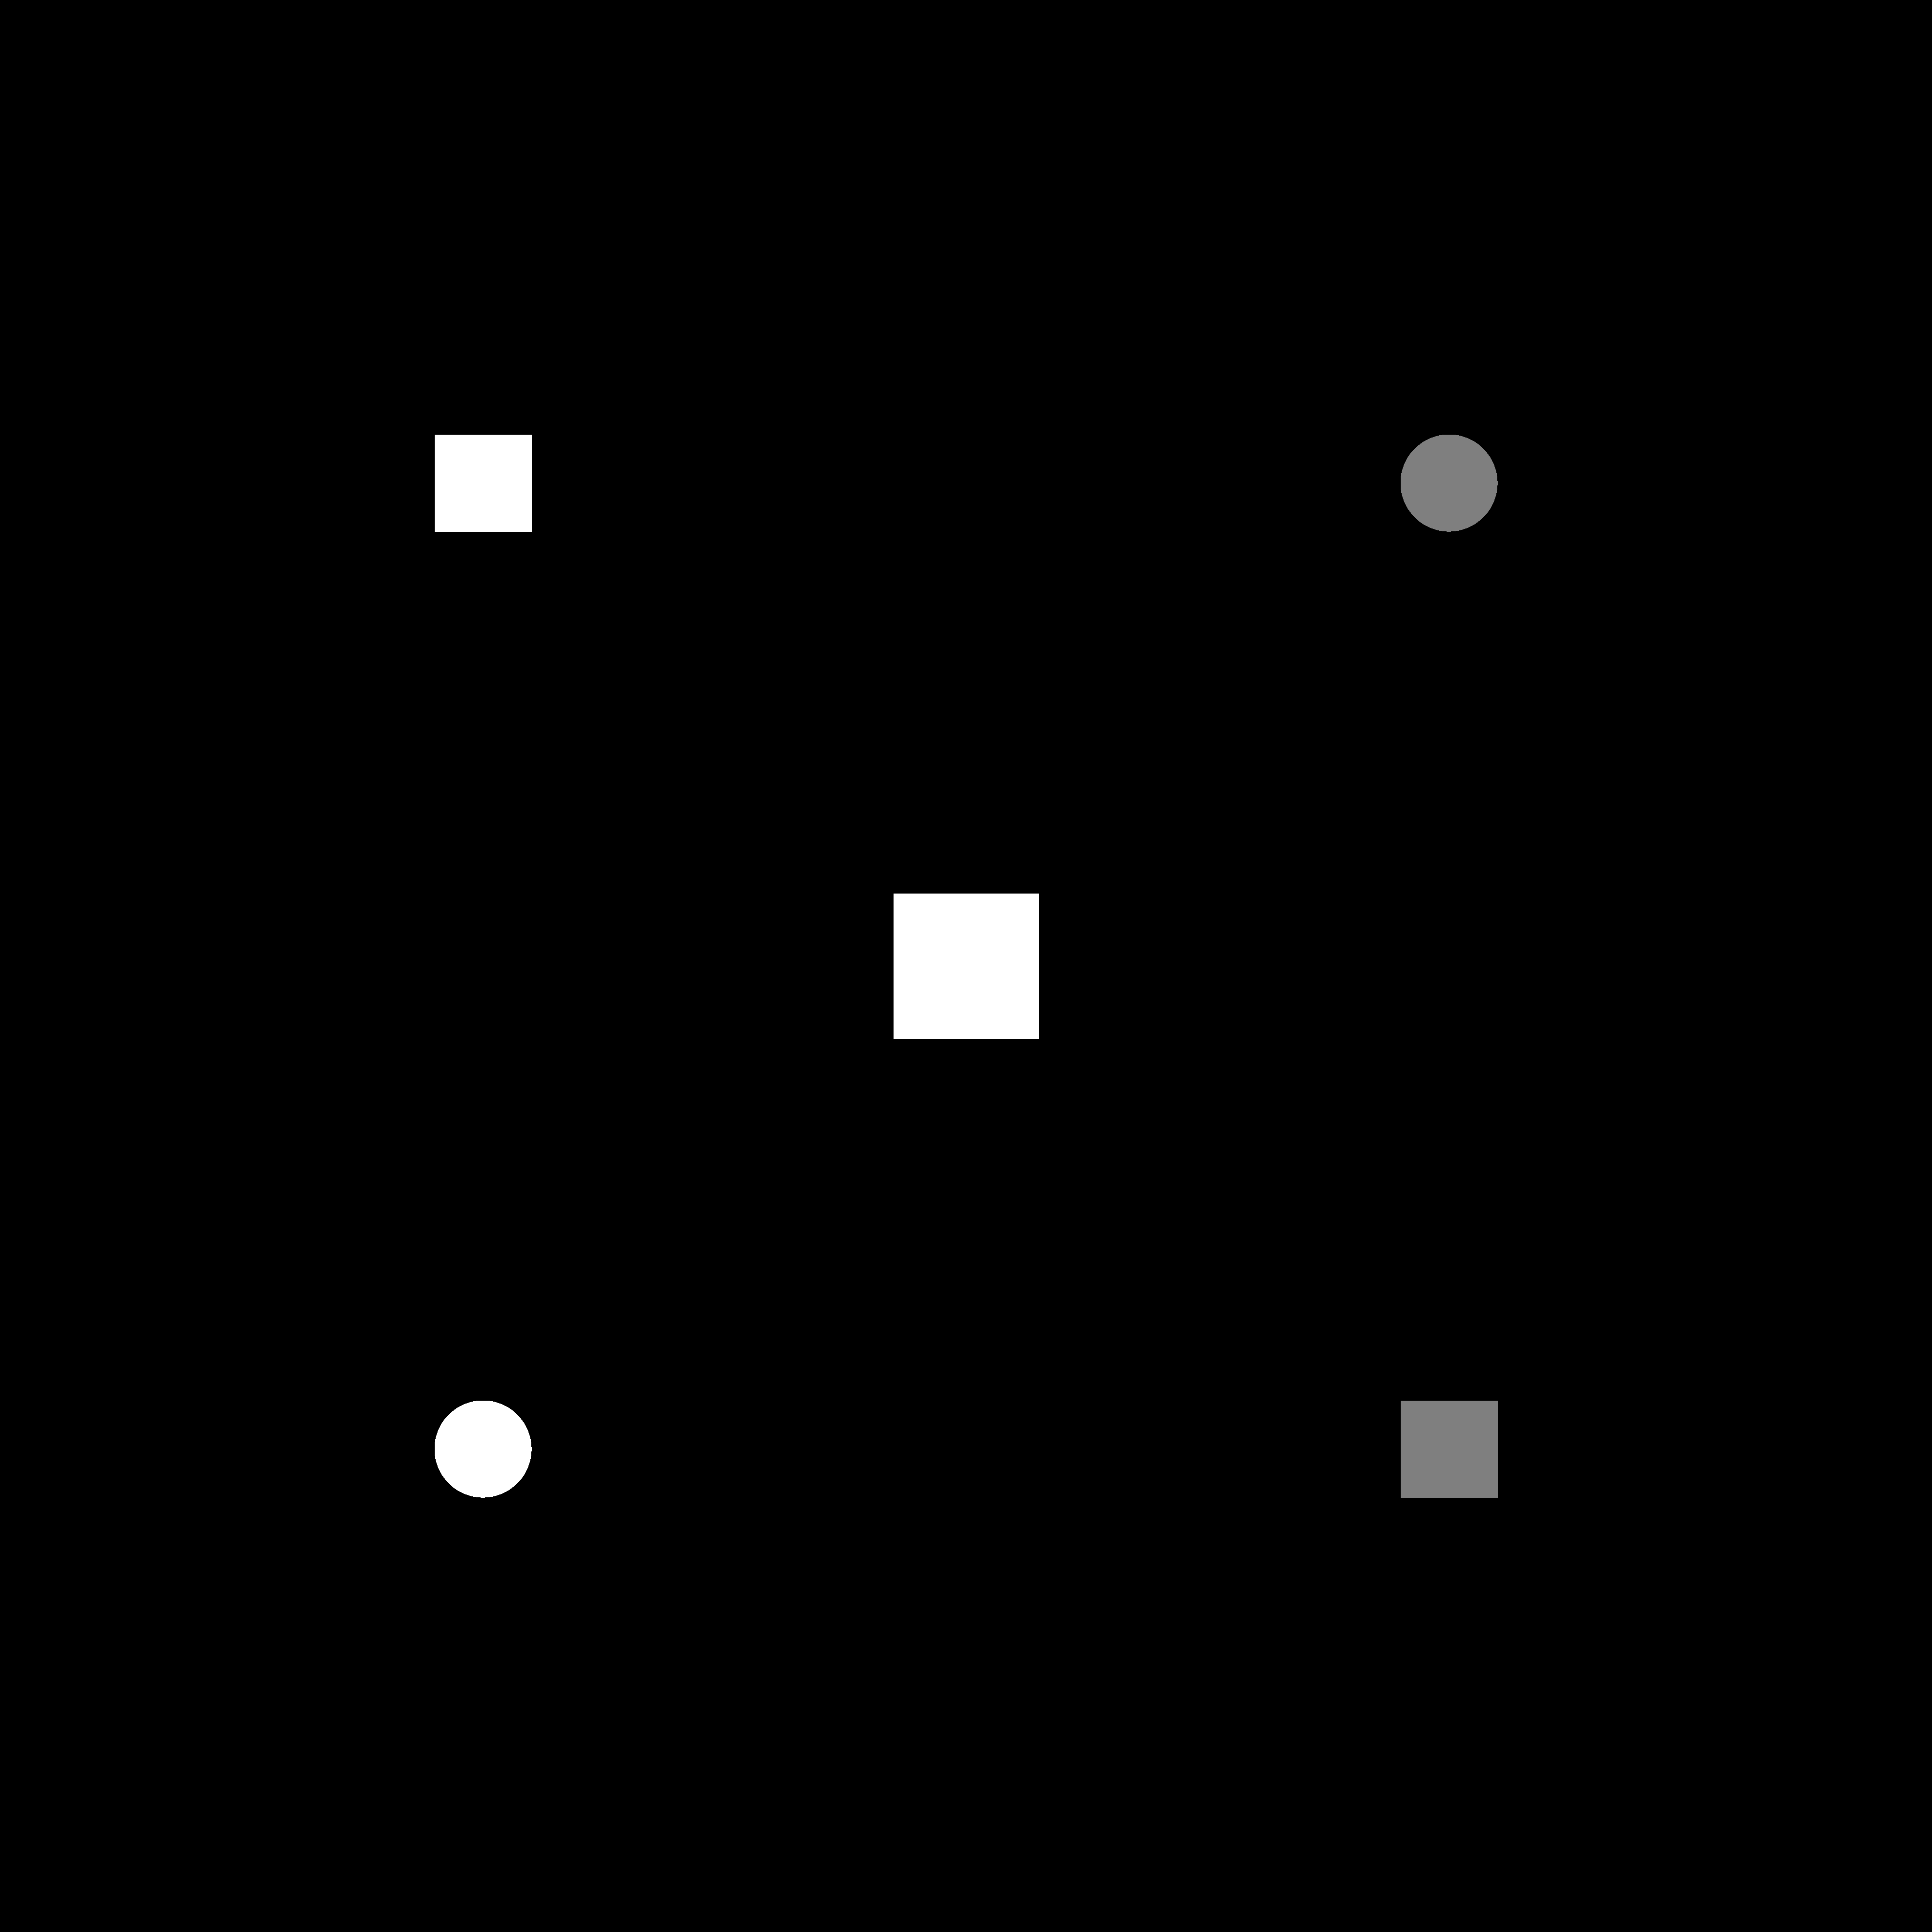
\includegraphics[scale=0.04]{images/toy_example.png}
	\end{figure}
	\vfill
\end{frame}

\begin{frame}[fragile]{SLDC: toy example (cont'd)}
\begin{minted}[fontsize=\scriptsize]{python}
# Defining a segmenter
class CustomSegementer(Segmenter):
    """All non-black pixels are in an object of interest"""
    def segment(self, image):
        return (image > 0).astype(np.uint8)
        
# Defining a dispatching rule 
class CircleRule(DispatchingRule):
    """A rule which matches circle polygons"""
    def evaluate_batch(self, image, polygons):
        return [circularity(p) > 0.85 for p in polygons]

# Defining a polygon classifier
class ColorClassifier(PolygonClassifier):
    """
    A classifier which returns the color (greyscale) 
    of the center pixel of the object
    """
    def predict_batch(self, image, polygons):
        classes = [center_pxl_color(image, p) for p in polygons]
        probas = [1.0] * len(polygons)
        return classes, probas
\end{minted}
\end{frame}

\begin{frame}[fragile]{SLDC: toy example (cont'd)}
\begin{minted}[fontsize=\scriptsize]{python}
# Build the workflow
builder = WorkflowBuilder()
builder.set_n_jobs(100)
builder.set_segmenter(CustomSegementer())
builder.add_classifier(CircleRule(), ColorClassifier(), disp_label="circle")
workflow = builder.get()

# Process an image
results = workflow.process(image)

# Go through the detected objects
for polygon, dispatch, label, proba in results:
  print "Detected polygon {}".format(polygon)
  print "Dispatched by '{}'".format(dispatch)
  print "Predicted class {}".format(label)
  print "Probability {}".format(proba)
  print ""
\end{minted}
\end{frame}

\begin{frame}[fragile]{SLDC: toy example (cont'd)}
\begin{minted}[fontsize=\scriptsize]{text}
Detected polygon POLYGON ((...))
Dispatched by 'circle'
Predicted class 128
Probability 1.0

Detected polygon POLYGON ((...))
Dispatched by 'circle'
Predicted class 255
Probability 1.0
\end{minted}
\end{frame}

\end{document}
